\section{Motivation}\label{sec:introduction:motivation}
% \dropcap{T}his is a introductory page.

% The last decades have shown great progress in robotics, with performant, precise, and powerful rigid robots now being widely adopted~\citep{todd1996fundamentals}, particularly in manufacturing scenarios where repetitive movements are prevalent within assembly line manufacturing, but more and more also in domains that require a larger degree of autonomy, such as warehouse logistics, automated inspections, etc.
% However, to address pressing societal challenges, there is a growing demand for robotic systems that are specifically designed for and adaptable to human-centered environments (e.g., homes and public spaces)~\citep{nahavandi2019industry, chibani2013ubiquitous, royakkers2015literature, he2021challenges}.
% To unlock their full potential, robots must be designed with inherent physical compliance to operate safely around humans in dynamic, unconstrained, unpredictable settings.
% Such requirement aligns with Asimov's First Law--robots must never harm humans--making safety fundamental to their design and deployment~\citep{villani2018survey}.
\dropcap{O}ver the past few decades, the domain of robotics has made remarkable strides, leading to the widespread adoption of high-performance, precise, and powerful rigid robots~\citep{todd1996fundamentals}. While these systems have traditionally excelled in manufacturing environments with repetitive tasks—such as assembly lines—they are increasingly finding use in applications that require more autonomy, including warehouse logistics and automated inspections. Yet, in addressing contemporary societal needs, there is a heightened demand for robots specifically crafted for human-centered settings, e.g., homes and public spaces~\citep{nahavandi2019industry, chibani2013ubiquitous, royakkers2015literature, he2021challenges}. Fully realizing the potential of such robots calls for integrating inherent compliance, enabling safe interaction with humans in dynamic, unconstrained, and unpredictable contexts. This requirement aligns with Asimov’s First Law~\citep{asimov1941three} — robots must never harm humans, making safety a paramount consideration in both their design and deployment~\citep{villani2018survey}.

% While safety is traditionally ensured through computational control policies, this approach is vulnerable to perception errors and often results in overly cautious behavior that limits robot performance. Soft robotics presents a promising alternative by establishing passive compliance throughout the entire robot body with material softness. This embodied intelligence is inherently resistant to perception or control
% errors. Recent years have witnessed remarkable progress in
% soft robotics, with researchers developing new designs, smart
% materials, actuators, sensors, models, and control approaches.

% Existing strategies mostly try to ensure safety via computational intelligence; for example, they advanced control mechanisms such as safety filters or impedance controllers, real-time collision detection, and predefined safety zones~\citep{zhao2024potential}. 
% For this task, they rely on sophisticated sensors, algorithms, and extensive pre-programming to anticipate and avoid hazards \citep{fragapane2021planning}.
% For example, collision detection enhances safety by stopping or slowing the robot upon contact. While reducing the worst-case injury likelihood, this approach is inherently reactive and cannot fully prevent injuries.
% However, in case of sensor failure or errors in the perception and/or reasoning pipeline, safety cannot be guaranteed anymore.
% There has also been work to improve safety through hardware.
% For example, \gls{Cobot}~\citep{el2019cobot}, designed to safely interact with humans, often use series elastic actuators to decouple the actuator from the link dynamics~\citep{pratt1995series} and aim to reduce the link inertia~\citep{albu2007dlr}.
% Yet, their rigid body still poses significant risks to nearby humans~\citep{haddadin2013towards}.
% In order to reduce safety risks, design standards such as ISO/TS 15066:2016~\citep{iso2016collaborative} demand that \gls{cobot} move slowly enough to stop in time to prevent collisions, limiting their effectiveness and performance~\citep{ajoudani2018progress, lucci2020combining}.
% In conclusion, the current strategies pose high requirements on perception systems and significantly reduce the robots/cobots' efficiency and effectiveness in the context of human-centered environments.
Existing approaches to ensuring safety largely depend on computational intelligence~\citep{ahn2024autort, sermanet2025generatingrobotconstitutions}, employing advanced control strategies, e.g., safety filters~\citep{ames2016control} and impedance controllers~\citep{khatib1987unified}, real-time collision detection~\citep{haddadin2017robot}, and predefined safety zones~\citep{zhao2024potential}. These methods leverage sophisticated sensing, algorithms, and extensive pre-programming to predict and mitigate potential hazards~\citep{fragapane2021planning}. For instance, collision detection improves safety by stopping or slowing the robot upon contact. Although this measure helps reduce the risk of serious injury, it is inherently reactive and cannot entirely eliminate harm. Moreover, any sensor malfunction or failure in the perception or decision-making pipeline undermines safety guarantees.
Hardware-based solutions have also been developed to enhance safety. For example, \glspl{Cobot}~\citep{el2019cobot}, which are designed for safe human-robot interaction, typically incorporate series elastic actuators to isolate actuator dynamics from the robot’s links~\citep{pratt1995series} and minimize link inertia~\citep{albu2007dlr}. Still, their rigid structures pose considerable risks to nearby individuals~\citep{haddadin2013towards}. To address these dangers, standards such as ISO/TS 15066:2016~\citep{iso2016collaborative} mandate that \glspl{Cobot} move slowly enough to stop before colliding with a person, thereby constraining performance and effectiveness~\citep{ajoudani2018progress, lucci2020combining}. Ultimately, current safety measures place heavy demands on perception systems and substantially reduce the efficiency and capabilities of robots and \glspl{Cobot} in human-centered environments.

\begin{figure}[ht]
    \centering
    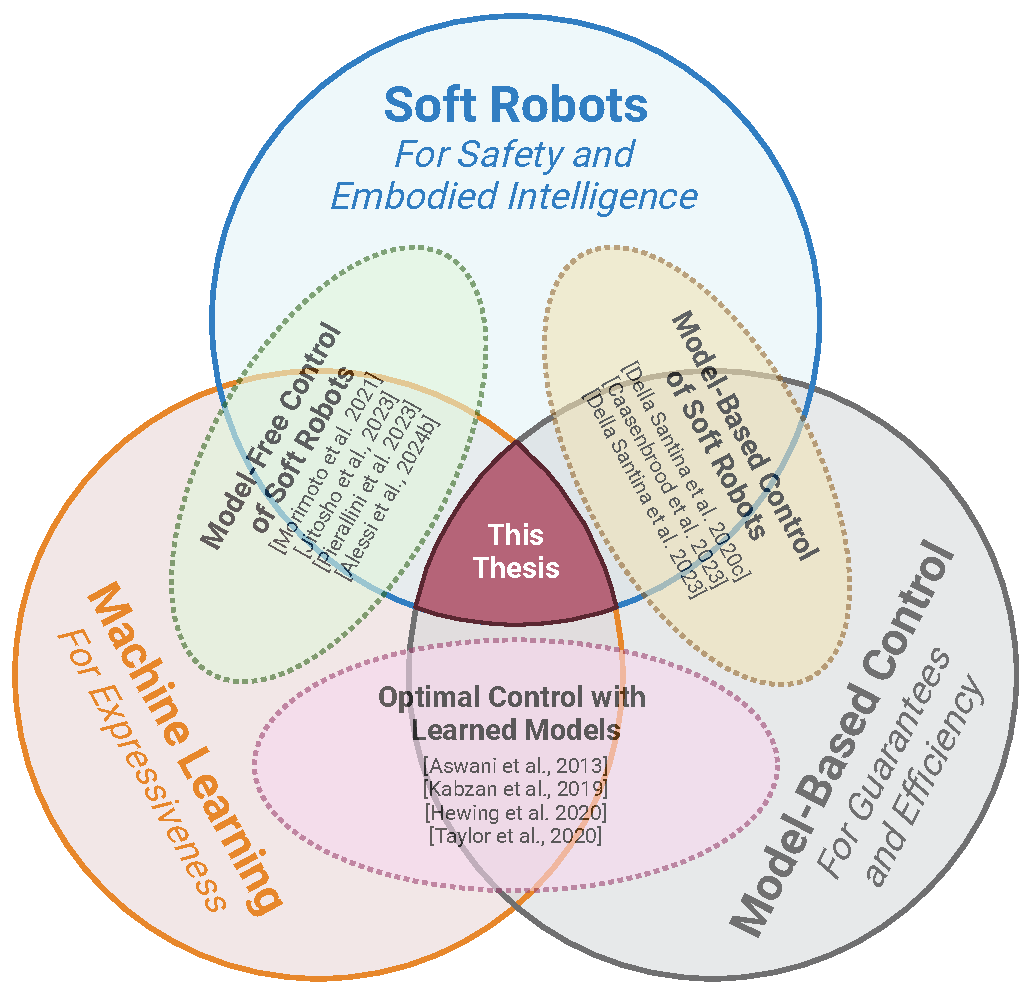
\includegraphics[width=0.8\linewidth]{introduction/figures/thesis_topics_venn_v2.pdf}
    \caption{Topics covered in this thesis: leveraging learned models for the control of soft robots.}
    \label{fig:introduction:topics_venn}
\end{figure}

% Interestingly, soft robotics redefines safety from the ground up. 
% In these robots~\citep{rus2015design, laschi2016soft}, safety is not an add-on or managed through computational stacks but is embedded in the material and structural properties of the robot itself. 
% Their compliant nature allows soft robots to interact safely with humans and operate in sensitive environments where safety is essential, such as personal assistance, caregiving, and handling delicate objects and produce~\citep{abidi2017intrinsic}. 
% Recent years have witnessed remarkable progress in soft robotics~\citep{yasa2023overview}, with researchers developing new designs~\citep{laschi2012soft, hawkes2017soft, guan2023trimmed, katzschmann2018exploration, tolley2014resilient}, smart materials~\citep{terryn2017self, mazzolai2022roadmap}, actuators~\citep{shepherd2013using, vasios2020harnessing, lipton2018handedness, gravert2024low, wehner2016integrated, aubin2022towards}, sensors~\citep{larson2016highly, thuruthel2019soft, truby2020distributed}, models~\citep{renda2018discrete, boyer2020dynamics, renda2020geometric}, and control~\citep{thuruthel2018model, della2020model, jitosho2023reinforcement, pustina2024input} approaches. 
% Despite their potential to revolutionize human-robot interaction~\citep{jorgensen2022soft}, soft robots face significant challenges hindering their full integration into practical applications~\citep{hawkes2021hard}. 
% Particularly, current soft robots often exhibit imprecise and often oscillatory motion~\citep{mazzolai2022roadmap, majidi2014soft, hawkes2017soft}.
% The reason is that modeling~\citep{armanini2023soft} and control~\citep{della2023model} of continuum soft robots presents significant challenges due to their infinite degrees of freedom, complex nonlinear dynamics, and time-dependent behaviors such as hysteresis.
Soft robotics reimagines safety from the ground up by embedding it into the robot’s fundamental mechanical design. Rather than treating safety as an add-on or relying solely on computational layers, soft robots incorporate safety through the choice of materials and structural configurations~\citep{rus2015design, laschi2016soft}. Their inherent compliance facilitates safe interactions with humans\footnote{
% We note, though, that the inherent safety of soft robots has, to the best of the author's knowledge, not yet rigorously quantified, experimentally analyzed and validated, for example, within controlled user studies, or compared to the safety of (collaborative) rigid manipulators. As a first step towards quantifying the (added) safety of soft robots, we propose a safety metric in Chapter~\ref{chp:safetymetric} of this thesis.
To the best of our knowledge, the inherent safety of soft robots has not yet been rigorously quantified, experimentally analyzed, or validated in literature—for instance, through controlled user studies or by comparing them to (collaborative) rigid manipulators. In Chapter~\ref{chp:safetymetric}, we introduce a safety metric as a first step toward quantifying the (added) safety of soft robots.
} 
and makes them ideal for safety-critical settings like personal assistance, caregiving, and handling delicate items~\citep{abidi2017intrinsic, yumbla2021human}.
Recent advances in the field have been substantial~\citep{yasa2023overview}, with innovations in soft robot designs~\citep{laschi2012soft, hawkes2017soft, guan2023trimmed, katzschmann2018exploration, tolley2014resilient}, smart materials~\citep{terryn2017self, mazzolai2022roadmap}, actuators~\citep{shepherd2013using, vasios2020harnessing, lipton2018handedness, gravert2024low, wehner2016integrated, aubin2022towards}, sensors~\citep{larson2016highly, thuruthel2019soft, truby2020distributed}, modeling methods~\citep{renda2018discrete, boyer2020dynamics, renda2020geometric}, and control techniques~\citep{thuruthel2018model, della2020model, jitosho2023reinforcement, pustina2024input}. Despite this progress and the potential to transform human-robot interaction~\citep{jorgensen2022soft}, widespread practical adoption of soft robots remains a challenge~\citep{hawkes2021hard}. In particular, many soft robots still struggle with imprecise, often oscillatory motion~\citep{mazzolai2022roadmap, majidi2014soft, hawkes2017soft}. This is largely because modeling~\citep{armanini2023soft} and controlling~\citep{della2023model} continuum soft robots from first principles is inherently difficult; they exhibit infinite degrees of freedom, complex nonlinear dynamics, and time-dependent phenomena such as hysteresis~\citep{armanini2023soft}, and might make extensive large-area multi-point contact with the environment.
% In summary, we find that current soft robots are not sufficiently capable, and specifically precise, which, similarly to safety-aware controllers for rigid robots that instill a very cautious and slow motion behavior, we are again paying performance for safety.
In summary, our findings indicate that current soft robots lack sufficient capability—particularly in precision—and, much like safety-aware controllers for rigid robots that enforce cautious, slow motions, we are again sacrificing performance for safety.
Therefore, we see a pressing need for novel motor control strategies for soft robots that combine the inherent compliance and embodied intelligence of soft robots with the precise motion characteristics of rigid robotic manipulators.

\begin{figure}[ht]
    \centering
    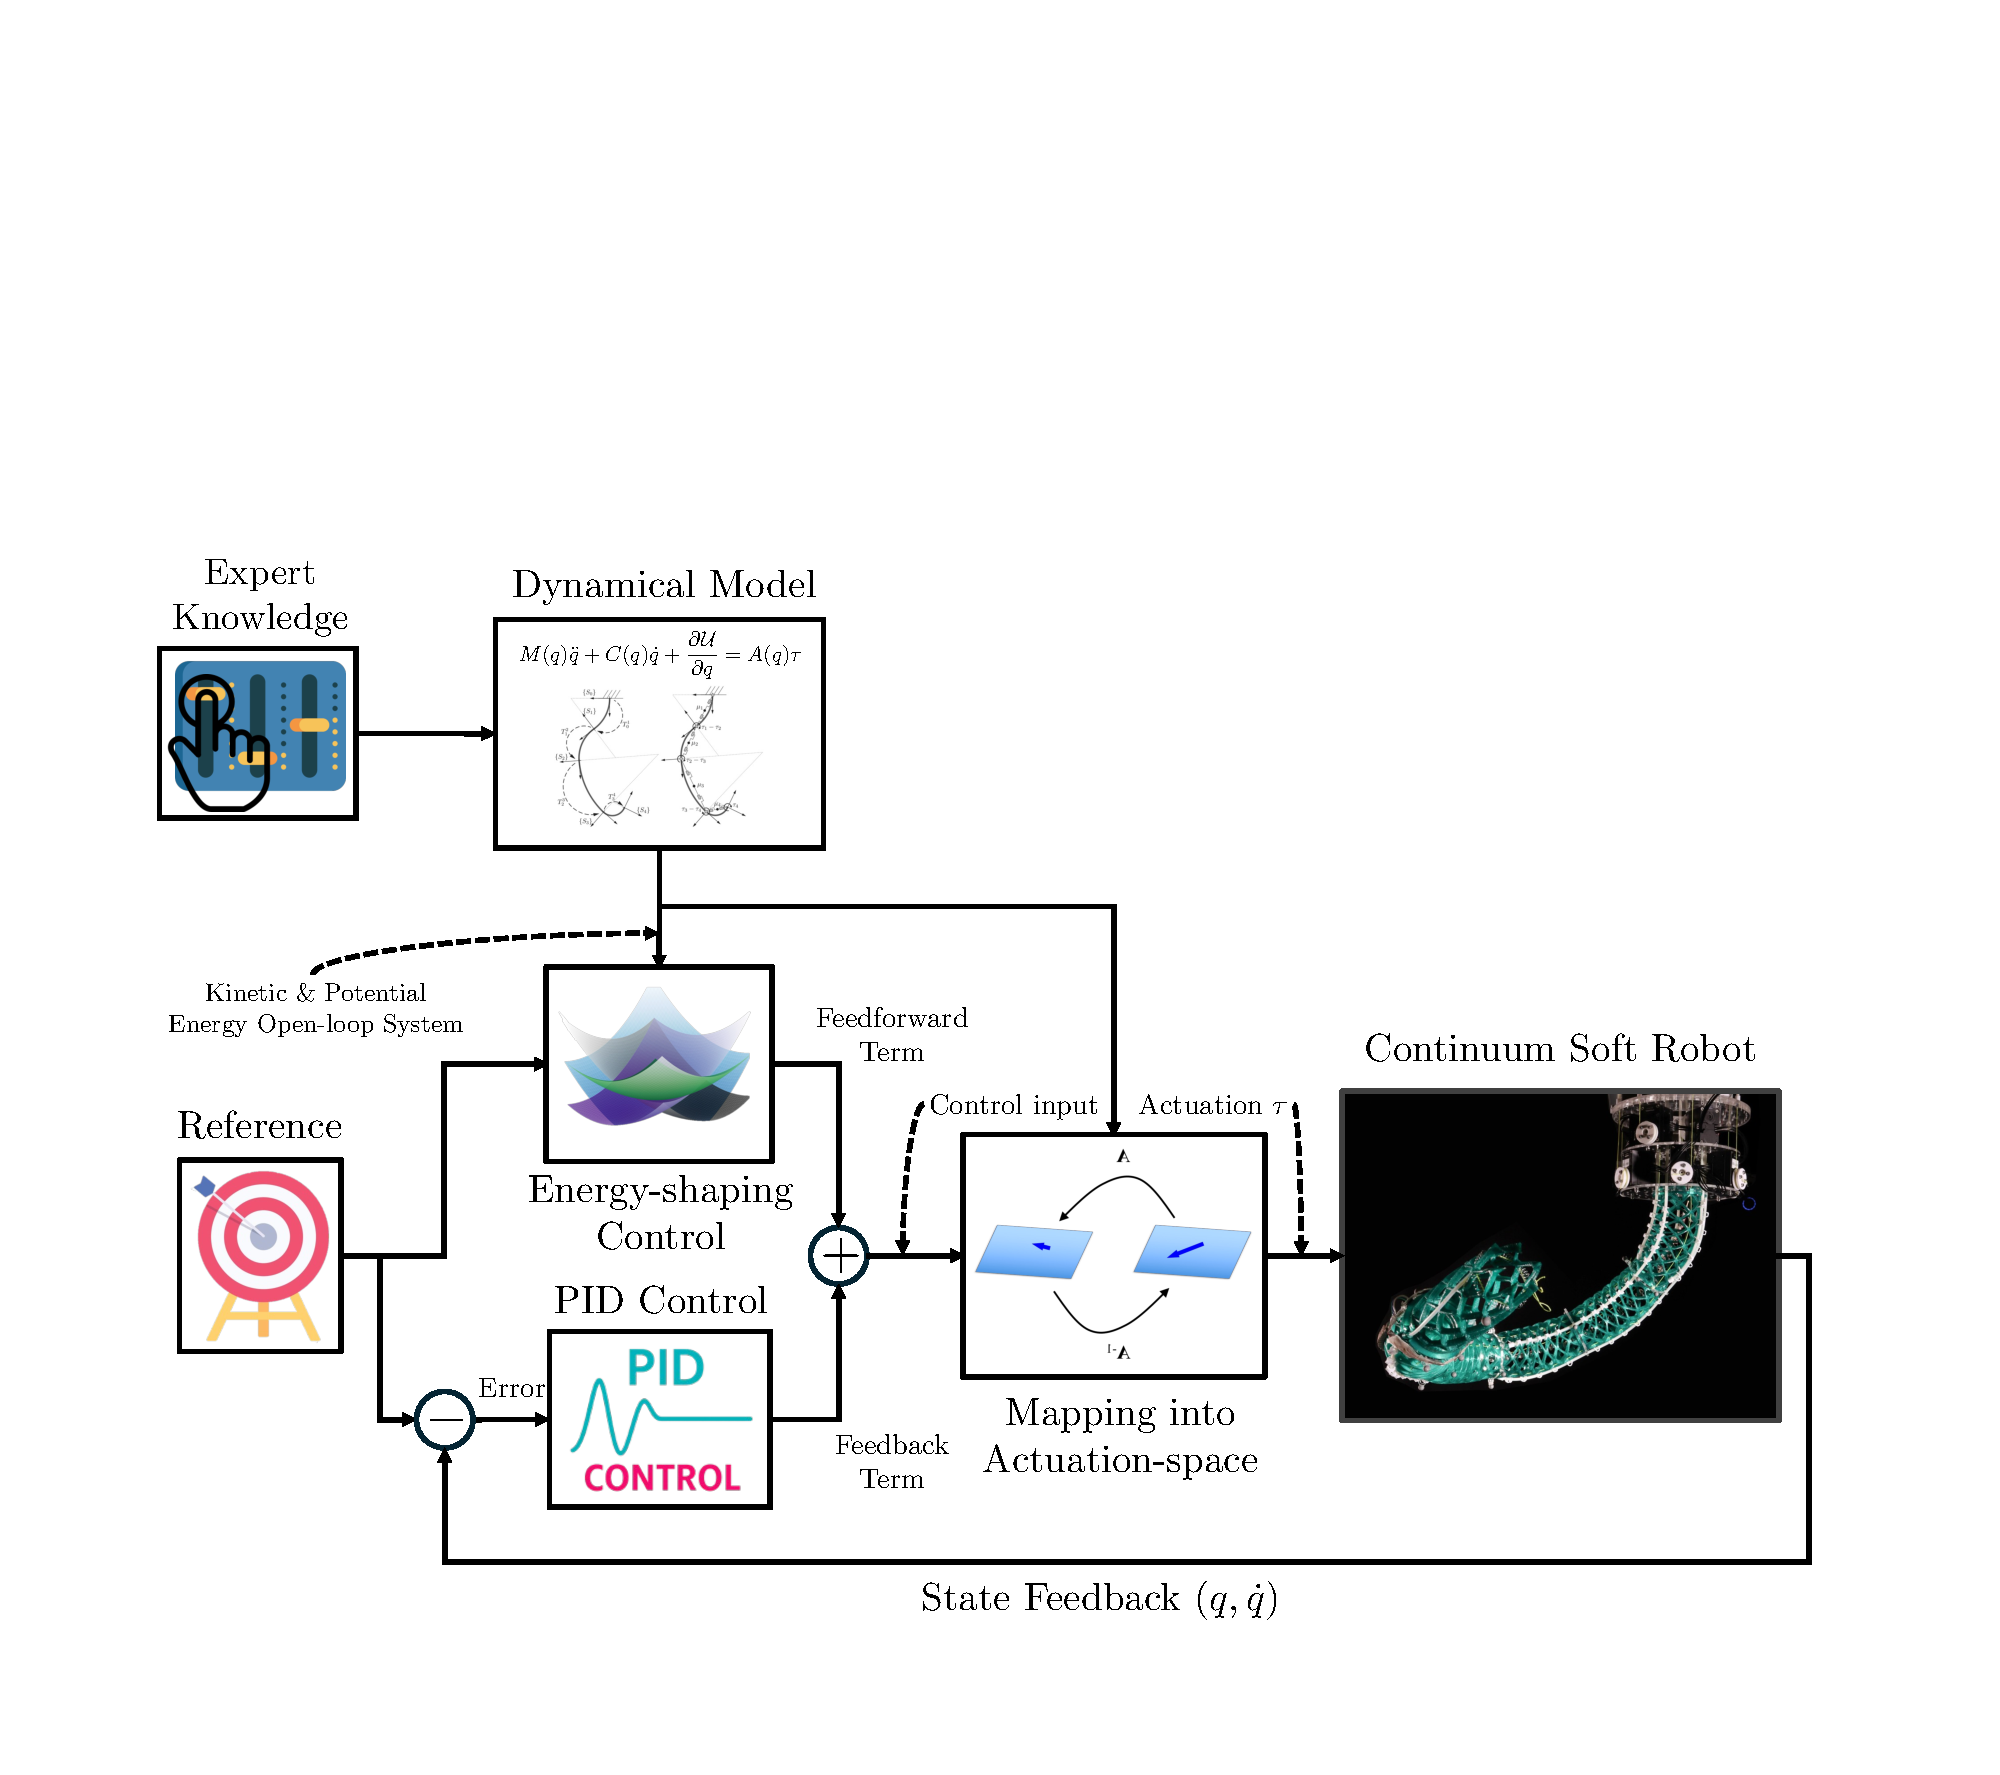
\includegraphics[width=1.0\linewidth]{introduction/figures/model_based_control_with_physical_models_v1_cropped.pdf}
    \caption{\textbf{Existing Approach: Model-Based Control with Physical Models.}
    % Derivation of physical models from first principles and subsequent usage within closed-form model-based control schemes, such as PID+energy-shaping~\cite{della2023model}.
    % Expert knowledge is needed to derive kinematic and dynamical models for soft robots from first principles. It is often possible to describe the dynamics in a control-oriented Euler-Lagrangian form. Subsequently, the model knowledge can be leveraged within closed-form controllers consisting of a feedback term (e.g., a PID-like controller) and a model-based term (e.g., an energy-shaping feedforward) that are tracking a given reference~\citep{della2023model}. Finally, the control input needs to be mapped into in an actuation that can be applied to the continuum soft robot in closed loop.
    Expert knowledge is required to derive kinematic and dynamic models for soft robots from first principles~\citep{armanini2017elastica}. The dynamics can often be expressed in a control-oriented Euler-Lagrangian framework. This model knowledge is then integrated into closed-form controllers that combine an error-based feedback term (e.g., a PID-like controller) with a model-based term (e.g., an energy-shaping feedforward) to track a given reference~\citep{della2020model, caasenbrood2021energy, della2023model}. Finally, the control input must be translated into an actuation that exerts forces and torques on the continuum soft robot in a closed loop.
    }
    \label{fig:introduction:model_based_control_with_physical_models}
\end{figure}

\begin{figure}[ht]
    \centering
    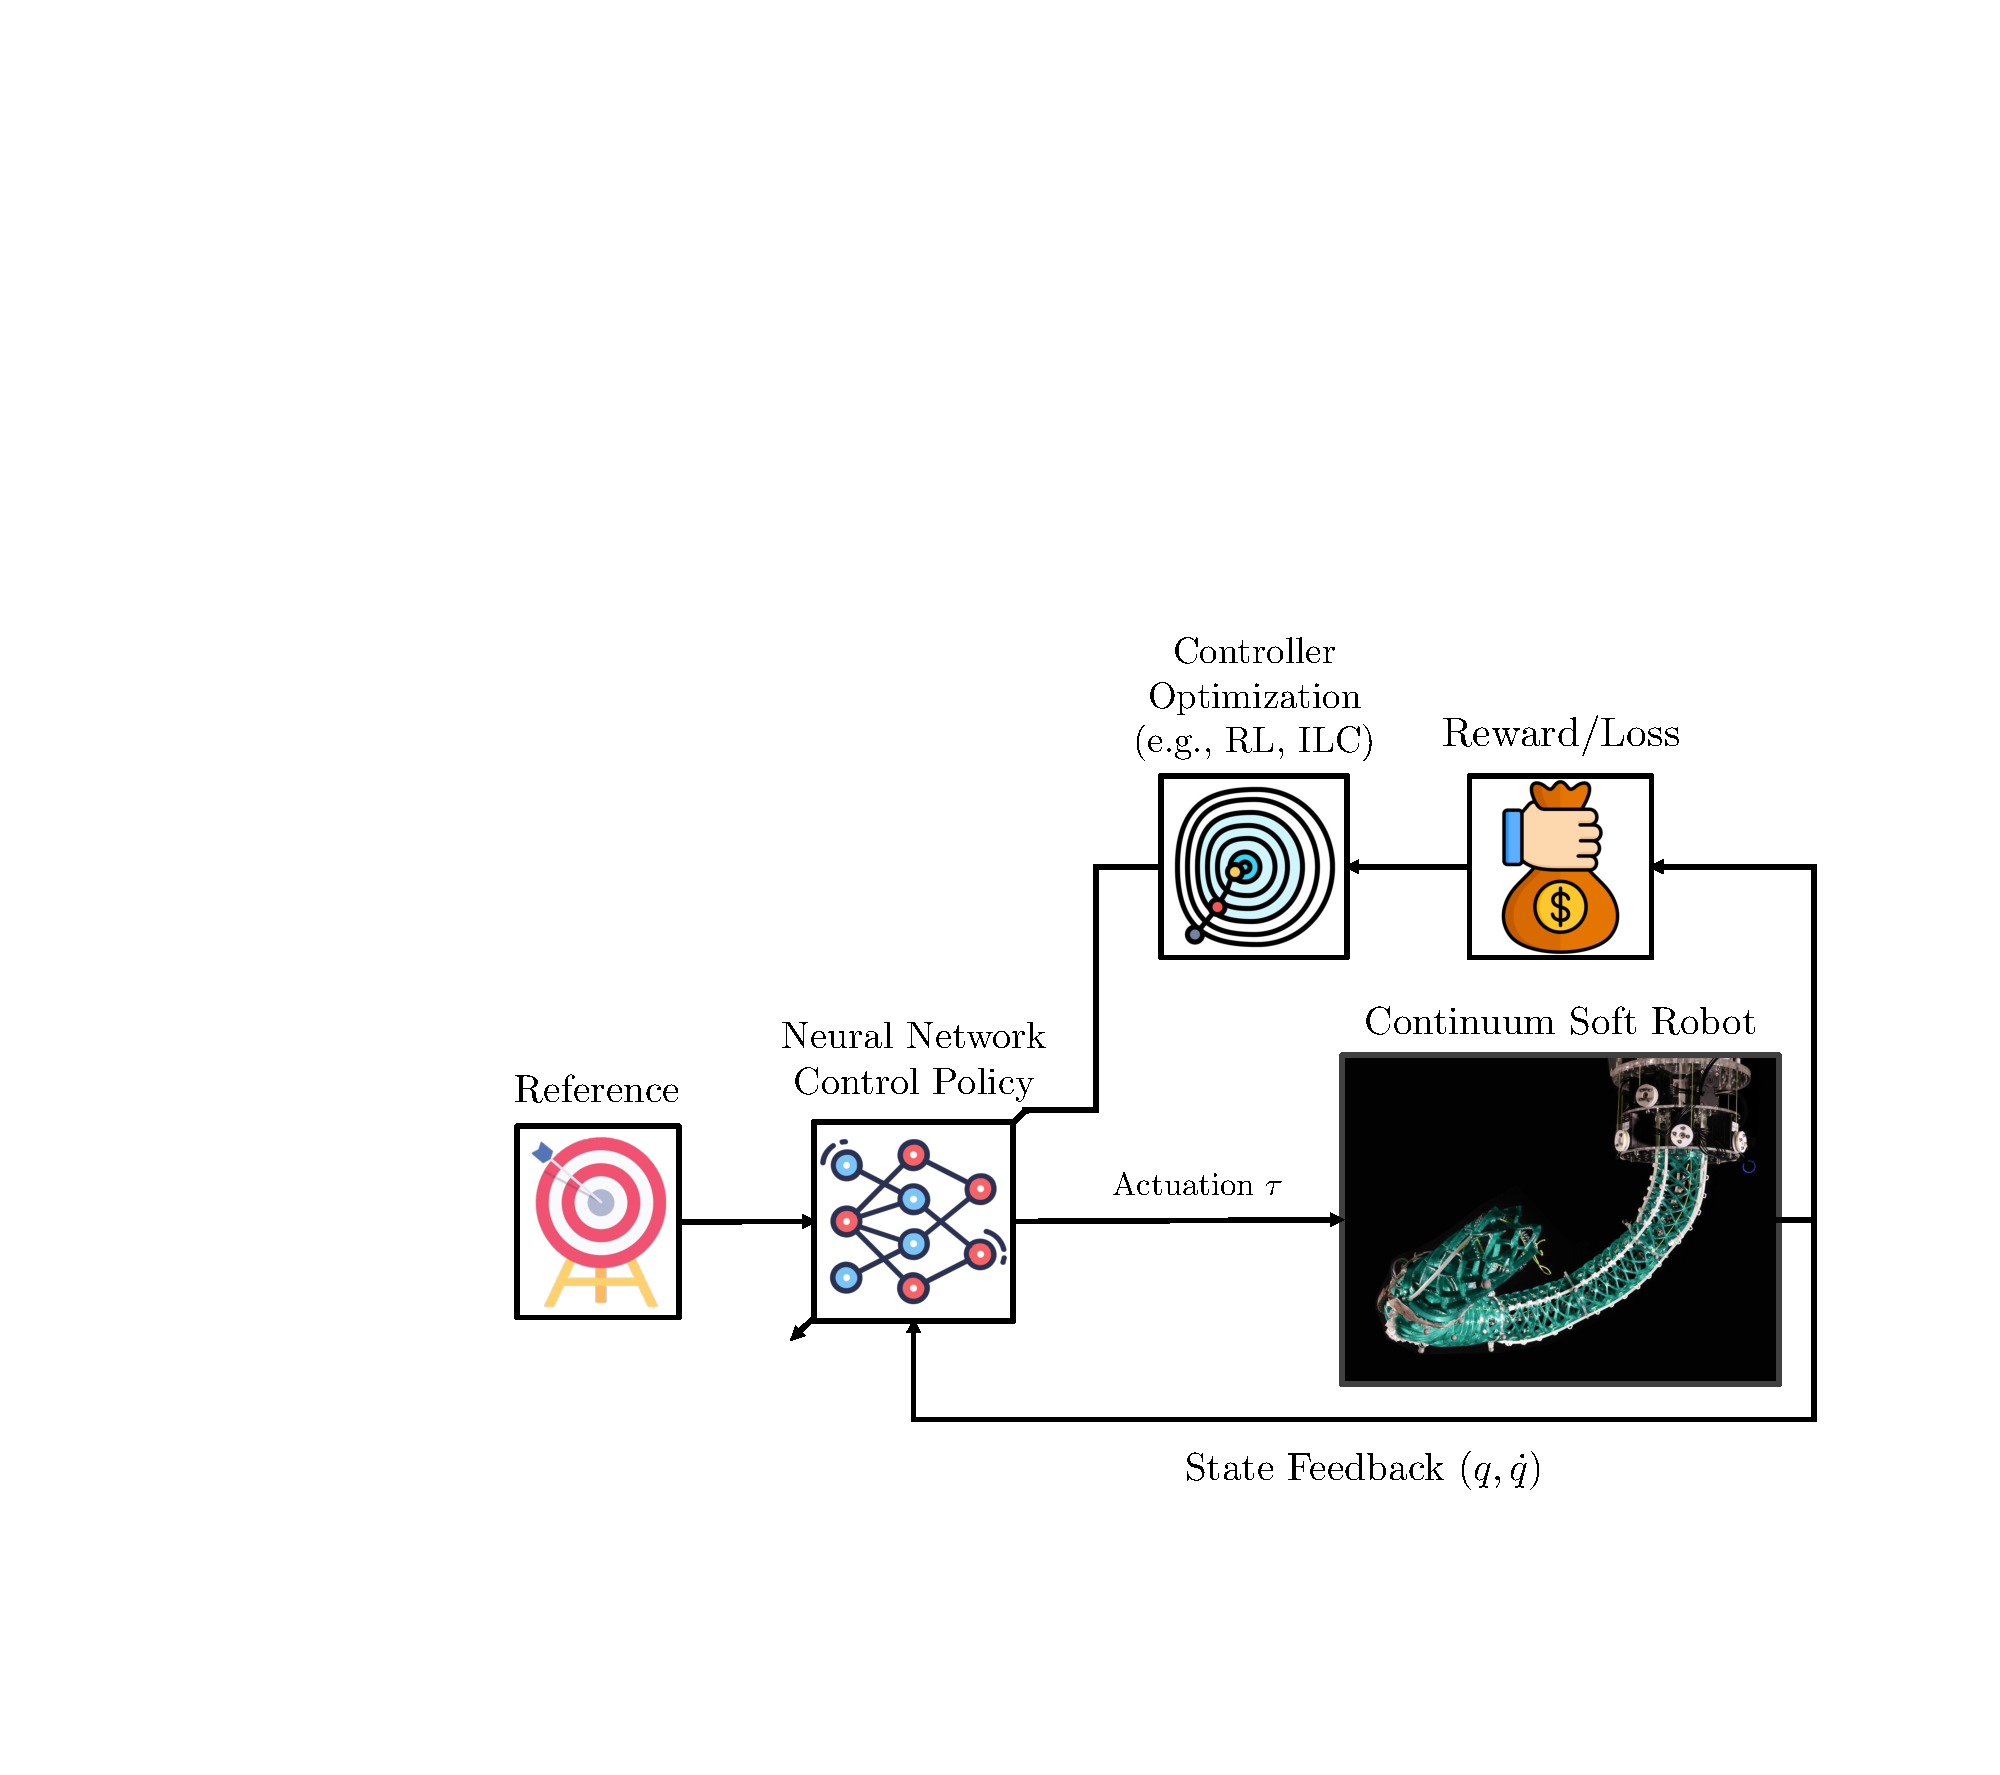
\includegraphics[width=0.75\linewidth]{introduction/figures/controller_learning_v1_cropped.pdf}
    \caption{\textbf{Existing Approach: Direct Controller Learning.} 
    Directly learning the controller via \gls{RL}~\citep{morimoto2021model, jitosho2023reinforcement, alessi2024pushing} or \gls{ILC}~\citep{hofer2019iterative, pierallini2023provably} by interacting with the soft robotic system and optimizing the control policy based on reward/loss/error signals.
    }
    \label{fig:introduction:direct_controller_learning}
\end{figure}

\begin{figure}[ht]
    \centering
    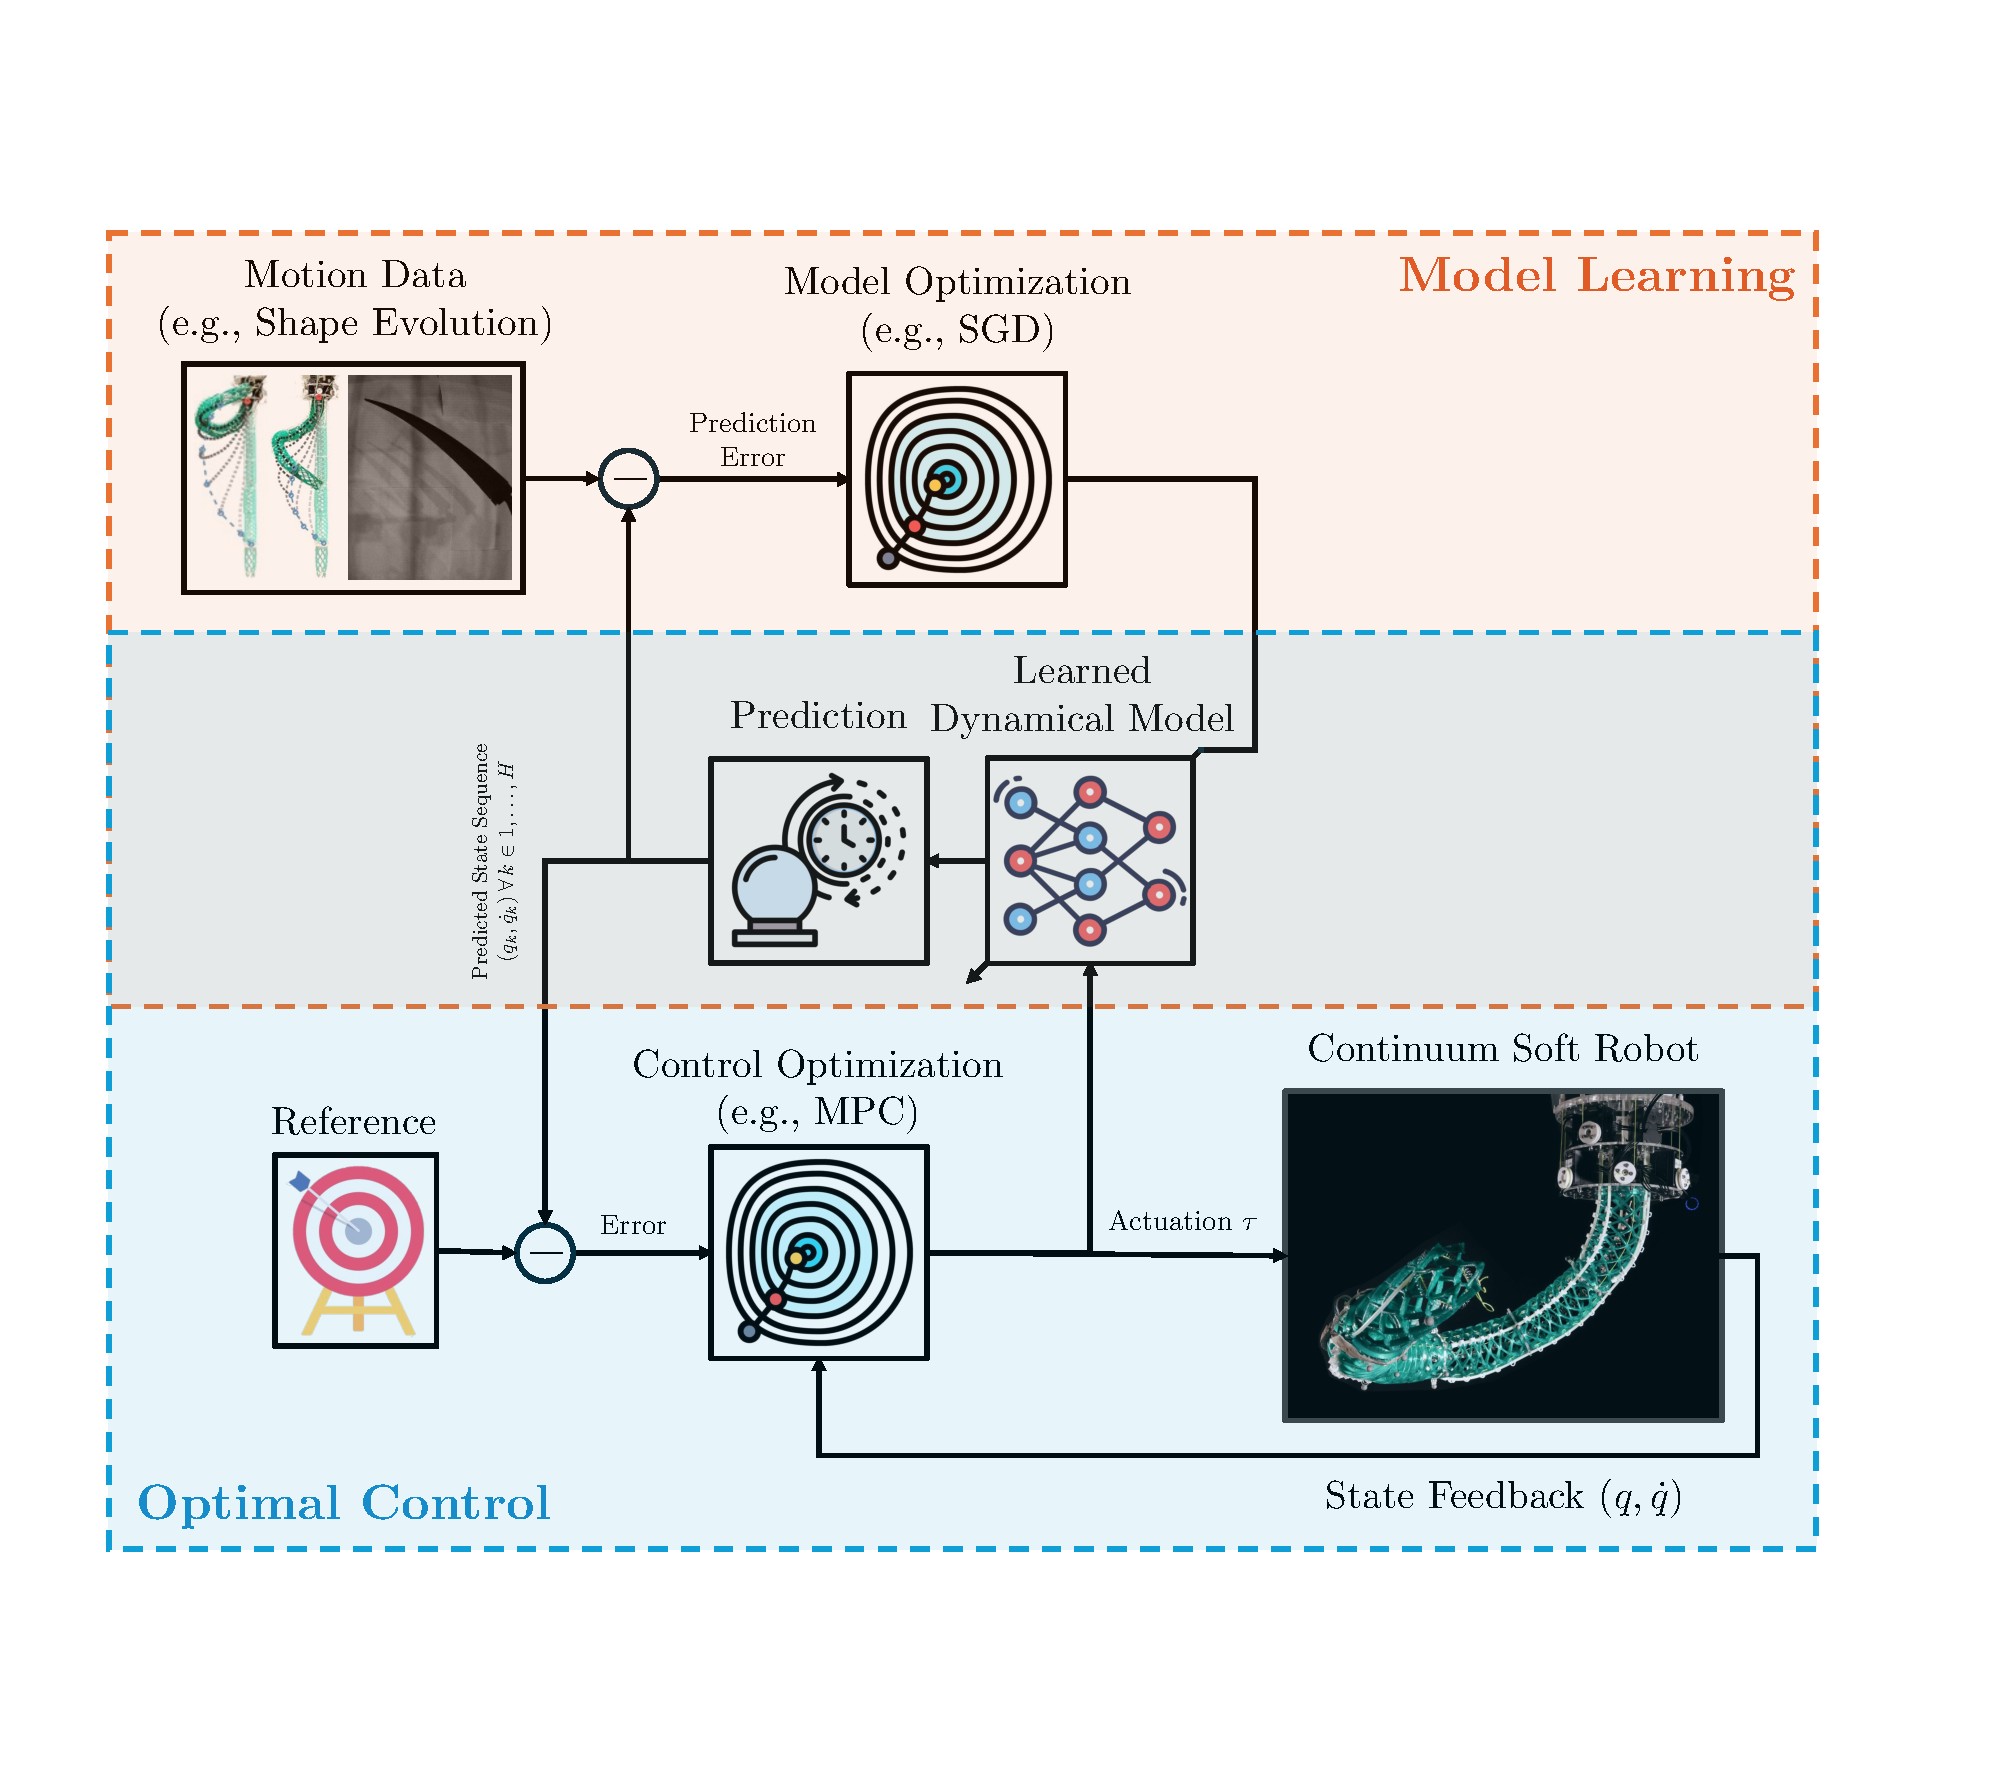
\includegraphics[width=0.9\linewidth]{introduction/figures/optimal_control_learned_models_v1_cropped.pdf}
    \caption{\textbf{Emerging Approach: Optimal Control with Learned Models.} 
    First, the dynamic model is learned via \gls{ML} approaches~\citep{gillespie2018learning, xie2023dynamic, alora2023data, alora2023robust, kasaei2023data, liu2024physics, chen2024data, marques2024visuo}, and subsequently, the control input is devised via optimal control techniques, such as \gls{LQR}~\citep{bruder2020data, bruder2024koopman} or \gls{MPC}~\citep{gillespie2018learning, hewing2020learning, alora2023data, alora2023robust}, by iteratively predicting the evolution of the closed-loop system for a given control input sequence over a horizon $H$ and using the error/loss between the predicted and desired behavior to optimize the control input.
    }
    \label{fig:introduction:optimal_control_with_learned_models}
\end{figure}

% At the moment, we can identify three dominant approaches for controlling the complex behavior of soft robots~\citep{thuruthel2018control, della2023model}:
% (1) leveraging fully physics-based models~\citep{armanini2023soft} (e.g., strain models~\citep{alessi2024rod}) for control, often using nonlinear feedback (e.g., PD+~\citep{della2020model}) or feedback+feedforward (e.g., PD+energy-shaping~\citep{della2023model, caasenbrood2023control} control schemes, (2) learning a model and subsequently exploiting it for control, be it via optimal control (e.g., \gls{LQR}~\citep{bruder2020data, haggerty2023control}, \gls{MPC}~\citep{gillespie2018learning, thuruthel2017learning, alora2023robust, alora2023data}, gradient-descent-based optimization~\citep{bern2020soft}), or model-based \gls{RL}~\citep{thuruthel2018model, centurelli2022closed}, or (3) directly learning the controller via model-free \gls{RL}~\citep{morimoto2021model, jitosho2023reinforcement, alessi2024pushing} or \gls{ILC}~\citep{hofer2019iterative, pierallini2023provably}.
% However, all strategies exhibit significant deficiencies and shortcomings:
At present, two main approaches can be distinguished for controlling the complex behavior of soft robots~\citep{thuruthel2018control, della2023model}. The first (1), visualized in Fig.~\ref{fig:introduction:model_based_control_with_physical_models}, relies on fully physics-based models~\citep{armanini2023soft}, for example using strain models~\citep{alessi2024rod}, and typically involves nonlinear feedback, e.g., PD+~\citep{della2020model}, or error-based feedback+feedforward, e.g., PID+energy-shaping~\citep{della2023model, caasenbrood2023control, soleti2025model}, control schemes. % The second (2) consists in learning a model and then exploiting it for control, whether through optimal control methods (e.g., \gls{LQR}~\citep{bruder2020data, haggerty2023control}, \gls{MPC}~\citep{gillespie2018learning, thuruthel2017learning, alora2023robust, alora2023data}, or gradient-descent-based optimization~\citep{bern2020soft, marques2024visuo}) or via model-based \gls{RL}~\citep{thuruthel2018model, centurelli2022closed}. 
The second (2) approach, visualized in Fig.~\ref{fig:introduction:direct_controller_learning}, is to learn the controller directly in a model-free fashion~\citep{george2017learning}, for example, through model-free \gls{RL}~\citep{morimoto2021model, jitosho2023reinforcement, alessi2024pushing} or \gls{ILC}~\citep{hofer2019iterative, pierallini2023provably}. However, both of these strategies exhibit significant drawbacks.

% (1) the derivation and design of fully physics-based models requires a lot of expert knowledge~\citep{stella2023science} and many simplifying assumptions, such as that the continuum soft robot's body is \emph{slender} (i.e., the backbone radius is much smaller than its length)~\citep{cosserat1909theorie} and can be approximated effectively by a low-dimensional kinematic parametrization~\citep{armanini2023soft}, backbone cross-sections preserve a constant area~\citep{gazzola2018forward}, the material is isotropic, exhibits Hookean behavior and does not display time-dependent characteristics such as hysteresis, etc. As a result, fully physics-based models do not sufficiently capture the complex behavior of advanced soft robots, which in turn leads to unsatisfactory of control performance.
% Approach (2) - learning linear dynamical models, for example, following a Koopman approach~\citep{bruder2020data, bruder2024koopman} such that they can be controlled via \gls{LQR} is often unstable, exhibits an inherent trade-off between dimensionality and expressiveness, and cannot accurately capture the behavior of non-linearizable systems~\citep{cenedese2022data}. On the other hand, learning the dynamics using nonlinear functions, and in particular \glspl{DNN}, for example, with \glspl{MLP}, \glspl{RNN}~\citep{thuruthel2018model, sun2022physics}, \glspl{LSTM}~\citep{xie2023dynamic}, or \glspl{NODE}~\citep{kasaei2023data} is a more expressive approach, but control becomes computationally very expensive techniques such as \gls{MPC} or model-based \gls{RL} need to be used. Furthermore, we usually lack a physical interpretation of the learned model, preventing us from analyzing the stability of the open-loop or closed-loop system using standard techniques, such as Lyapunov arguments~\citep{khalil2002nonlinear}.
% The third existing approach, (3), in the case of \gls{RL} sample inefficient and lacks stability guarantees, and in the case of \gls{ILC} can only learn repetitive trajectories~\citep{bristow2006survey}.
% In particular, the sample inefficiency is a huge issue for soft robots as they exhibit changing material properties rendering previously learned controllers to be suboptimal, and a currently a limited lifetime~\citep{yasa2023overview} - which might mean that the soft robot might be damaged or broken before the (\gls{RL}) controller is fully trained.
Developing fully physics-based models, as used in (1), demands substantial expert knowledge~\citep{stella2023science} and often hinges on strong simplifying assumptions, such as the continuum soft robot being slender, i.e., the backbone radius is much smaller relative to its length~\citep{cosserat1909theorie}, allowing for a low-dimensional kinematic parametrization~\citep{armanini2023soft}, preserving a constant backbone cross-section~\citep{gazzola2018forward}, and assuming isotropic Hookean materials without time-dependent effects like hysteresis. These assumptions fail to capture the intricate physics of many soft robots, undermining control performance. 
% Furthermore, it seems currently infeasible to model the joint dynamics of a soft robot interacting intensively with the world around it (e.g., collaborating with humans, being in contact with the environment over large-areas at multiple points along the body, predicting the evaluation of the world in the spirit of world models~\citep{ha2018world}) accurately just using first principles from physics therefore motivating the need to adapt learning-based solutions.
Furthermore, accurately modeling from physics using only first principles the joint dynamics of a soft robot that interacts intensively with the environment—whether by collaborating with humans, making extensive large-area multi-point contact with its surroundings, or predicting the environment dynamic evaluation in the spirit of world models~\citep{ha2018world}—appears currently infeasible, thereby motivating the need for learning-based solutions.
Discussing approach (2): Model-free \gls{RL}, meanwhile, tends to be sample inefficient and does not guarantee stability, whereas \gls{ILC} can only be used for learning repetitive trajectories~\citep{bristow2006survey}. The sample inefficiency is particularly problematic for soft robots since their material properties change over time—rendering previously learned controllers less effective—and their limited lifespans~\citep{yasa2023overview} risk the robot being damaged or failing altogether before a controller learned through \gls{RL} is fully trained.
The lack of insight into the decision-making process and the lack of stability guarantees can cause safety issues, particularly when operating in close proximity to humans.

% To counteract the disadvantages of approaches (1) and (2), there have been in recent years steps to combine the benefits of \gls{ML} and model-based control by first learning a model, for example, using a \gls{NN}, and subsequently exploiting it for control.
% However, this increase of model expressiveness through \gls{ML} techniques has come at the cost of computational control efficiency as closed-form controllers are usually not available, and we need to resort to optimization-based strategies.
To overcome the limitations of approaches (1) and (2), research in recent years has combined the strengths of \gls{ML} and model-based control by first learning a model—often using a \gls{NN}—and then exploiting it for control~\citep{gillespie2018learning, thuruthel2018model, bruder2020data, bruder2024koopman, alora2023data, alora2023robust, chen2024data}. However, this enhanced model expressiveness through \gls{ML} techniques comes at the expense of computational efficiency, as closed-form controllers are typically unavailable, and one must rely on optimal control/optimization-based strategies (see Fig.~\ref{fig:introduction:optimal_control_with_learned_models}).
For example, learning linear dynamical models—such as those based on a Koopman approach~\citep{bruder2020data, bruder2024koopman} often proves unstable, suffers from the trade-off between model dimensionality and expressiveness, and cannot accurately represent non-linearizable systems~\citep{cenedese2022data}. On the other hand, using nonlinear functions (notably \glspl{DNN}, including \glspl{MLP}, \glspl{RNN}~\citep{thuruthel2018model, sun2022physics}, \glspl{LSTM}~\citep{xie2023dynamic}, or \glspl{NODE}~\citep{kasaei2023data} provides more expressive models but requires computationally heavy control techniques such as optimal control with \gls{MPC}~\citep{gillespie2018learning, aswani2013provably, kabzan2019learning, hewing2020learning, alora2023data, alora2023robust} or \glspl{CBF}~\citep{taylor2020learning}, or model-based \gls{RL}~\citep{thuruthel2018model} as they typically lack a clear physical structure that would allow, for example, for energy shaping-based or feedback-linearization control~\citep{khalil2002nonlinear} and that would permit stability analyses of both the open-loop and closed-loop system by conventional means, such as Lyapunov arguments~\citep{khalil2002nonlinear}. 
% The high computational demand required for \gls{MPC} limits the maximum control frequence that can be realized in practice - therefore also limiting the ability to control highly dynamic behaviors effectively.
The high computational demand associated with \gls{MPC} limits the maximum control frequency achievable in practice, thereby restricting the effective control of highly dynamic behaviors.

\begin{figure}[ht]
    \centering
    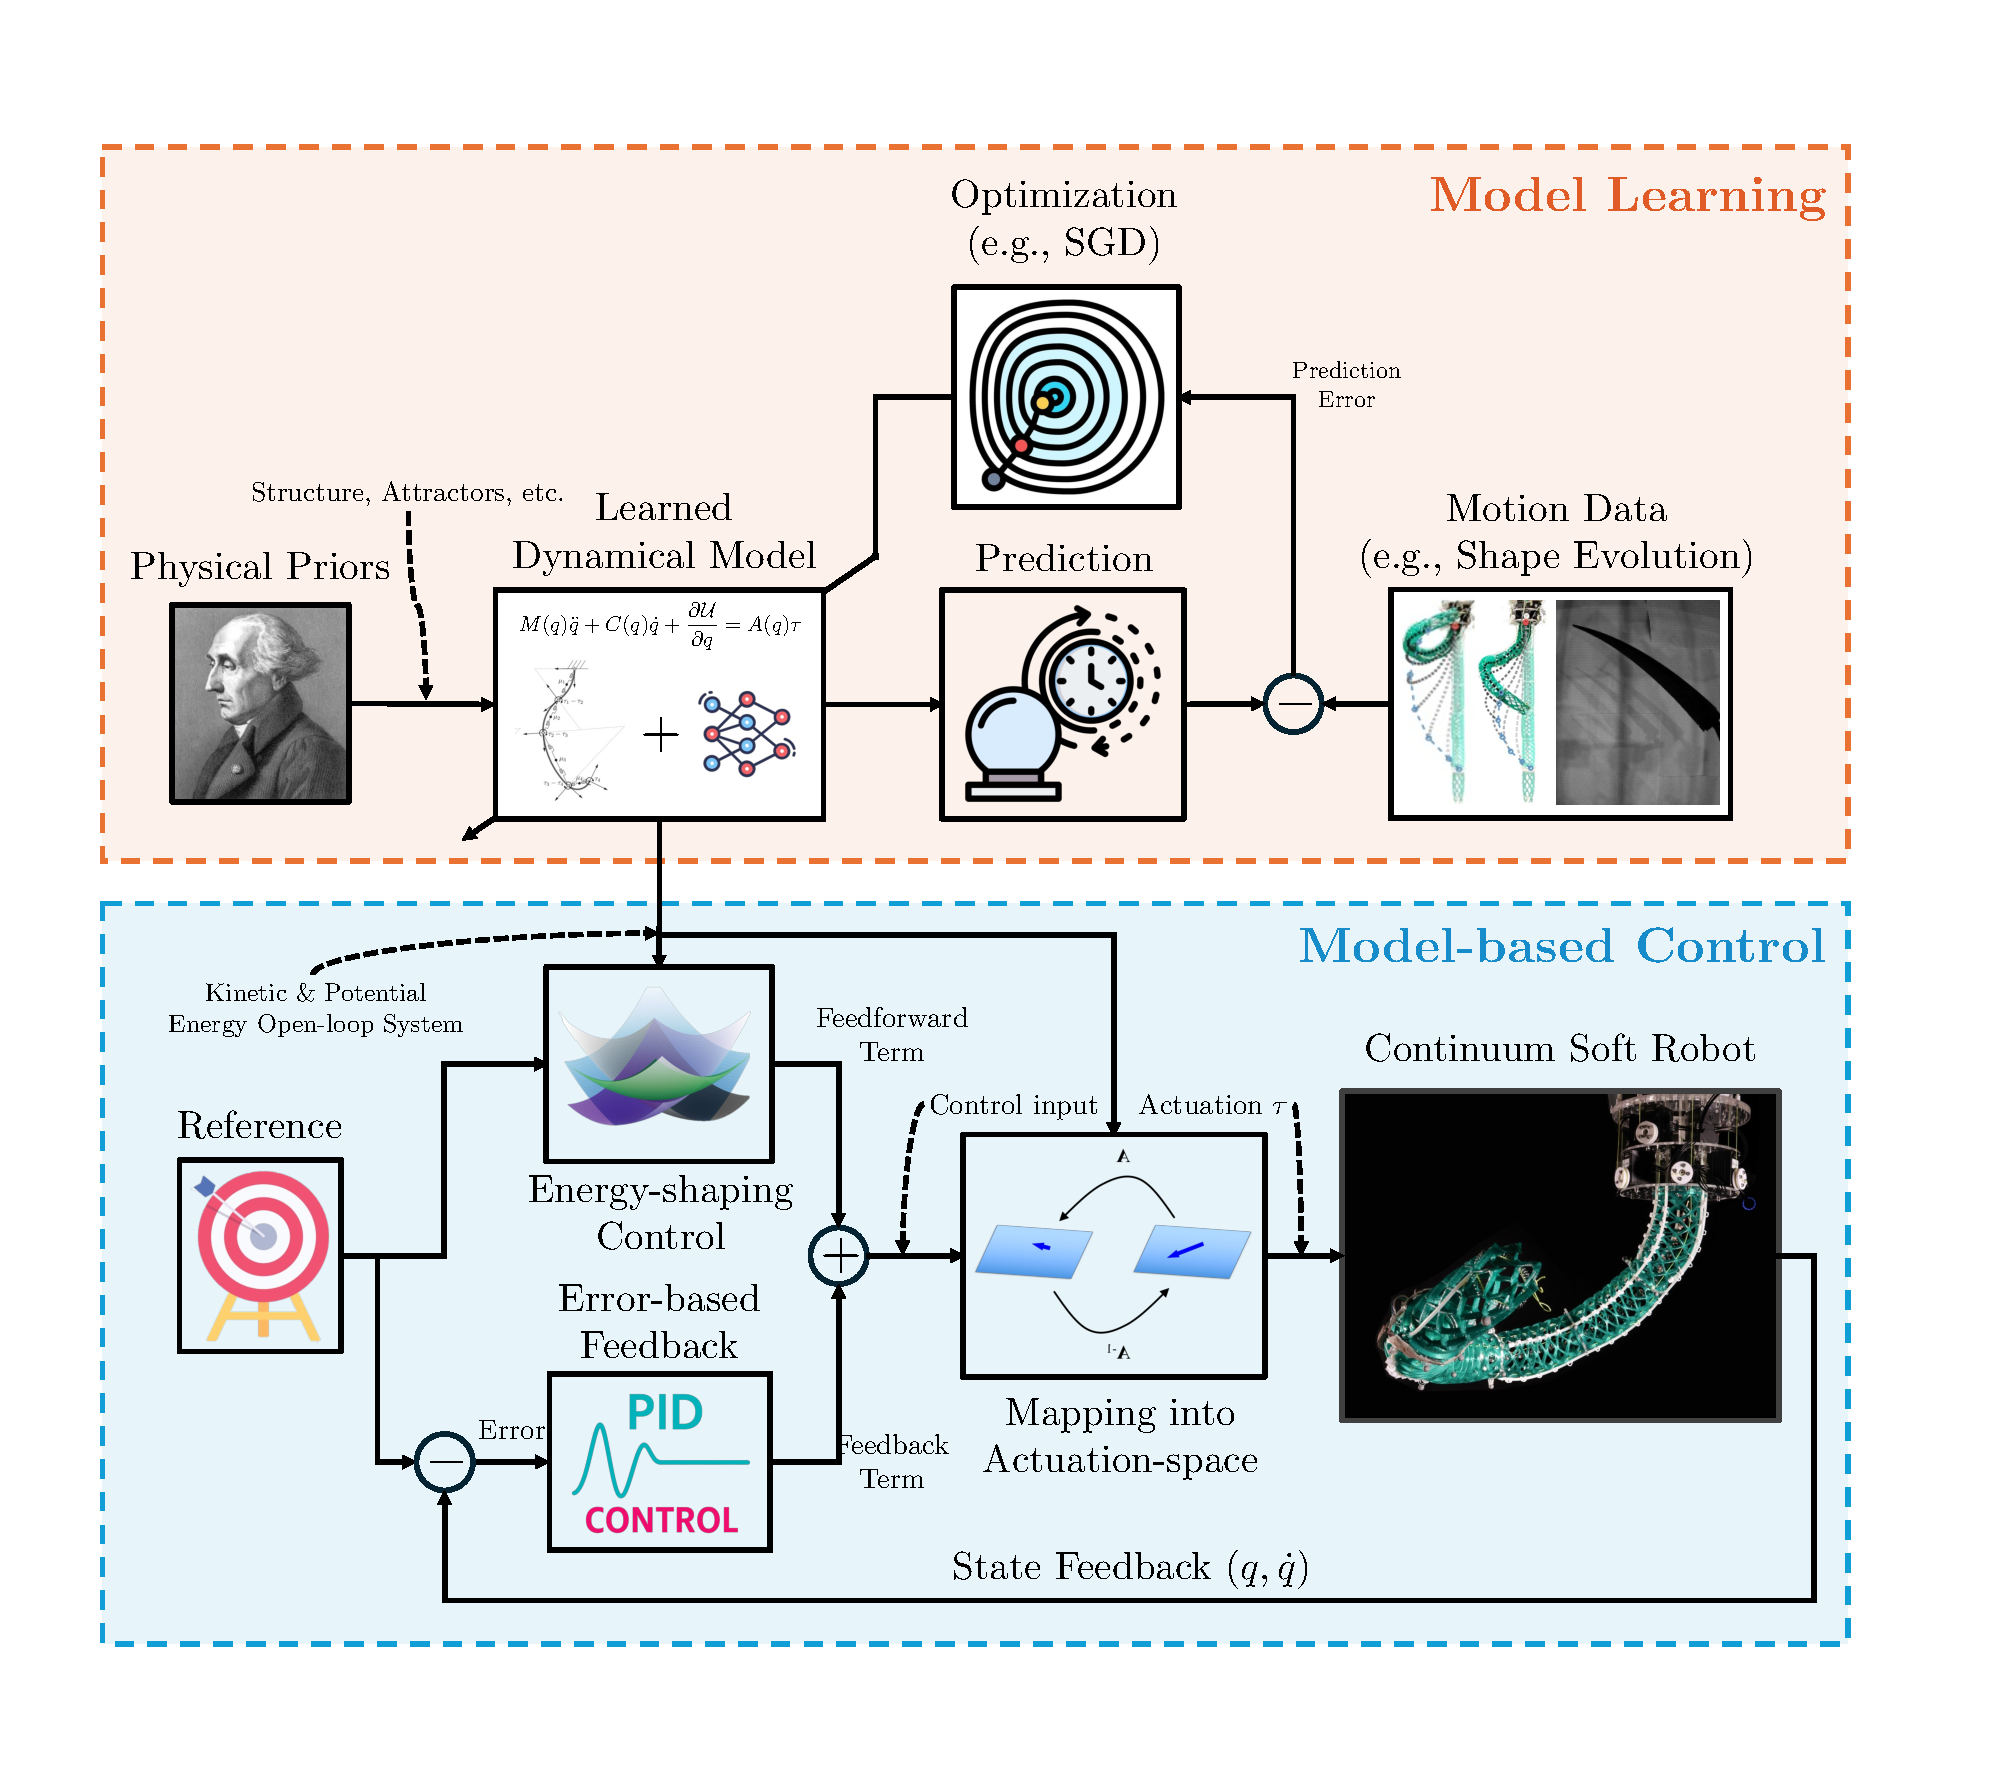
\includegraphics[width=0.9\linewidth]{introduction/figures/model_based_control_with_learned_models_v3_cropped.pdf}
    \caption{\textbf{Core Contribution of this Thesis.} 
    % Closed-form model-based control with learned models that exhibit a physical structure.
    % The core contribution of this thesis is to combine learned models with closed-form controllers. To make this possible, we learn the dynamical models with a physical structure which makes it possible for us to derive the potential and kinetic energy of the learned system. Apart from the specific structure of the dynamical model, the model learning follows a standard approach as established in literature by predicting the future evolution of the soft robotic system, comparing the prediction with a dataset of actual motion data, and using this prediction error to optimize the free parameters of the learned dynamical model.
    % Moving to control, we reshape the potential energy of the closed-loop system by adding a feedforward term that regulates the system towards a given reference~\citep{della2023model}. This potential shaping feedforward term is complemented by an integral-saturated PID feedback term, named P-satI-D~\citep{pustina2022p}, that rejects disturbances and compensates for modeling errors. Finally, the control input is mapped into an actuation, which is potentially also learned.
    % The insight into the potential and kinetic energy systems enables us to analyze the stability and convergence characteristics of both open-loop and closed-loop systems using Lyapunov arguments~\citep{khalil2002nonlinear}.
    The primary contribution of this thesis is the integration of learned models with closed-form controllers. To enable this, we learn dynamical models with a physical structure that allows us to derive the system’s potential and kinetic energy. Beyond the specific dynamical model structure, the learning process follows a well-established approach in the literature: we predict the future evolution of the soft robotic system, compare these predictions with actual motion data, and use the resulting prediction error to optimize the free parameters of the learned model.
    % 
    On the control side, we modify the closed-loop system’s potential energy by incorporating a feedforward term that steers the system toward a designated reference~\citep{della2023model}. This potential shaping feedforward is complemented by an integral-saturated PID feedback term, known as P-satI-D~\citep{pustina2022p}, which rejects disturbances and compensates for modeling errors. Finally, the control input is translated into an actuation signal, where this mapping may also be learned. This insight into the potential and kinetic energy permits an analysis of the stability and convergence properties of both open-loop and closed-loop systems using Lyapunov arguments~\citep{khalil2002nonlinear}.
    }
    \label{fig:introduction:model_based_control_with_learned_models}
\end{figure}

% \begin{figure}[ht]
%     \centering
%     \subfigure[Closed-form Control with Physical Models]{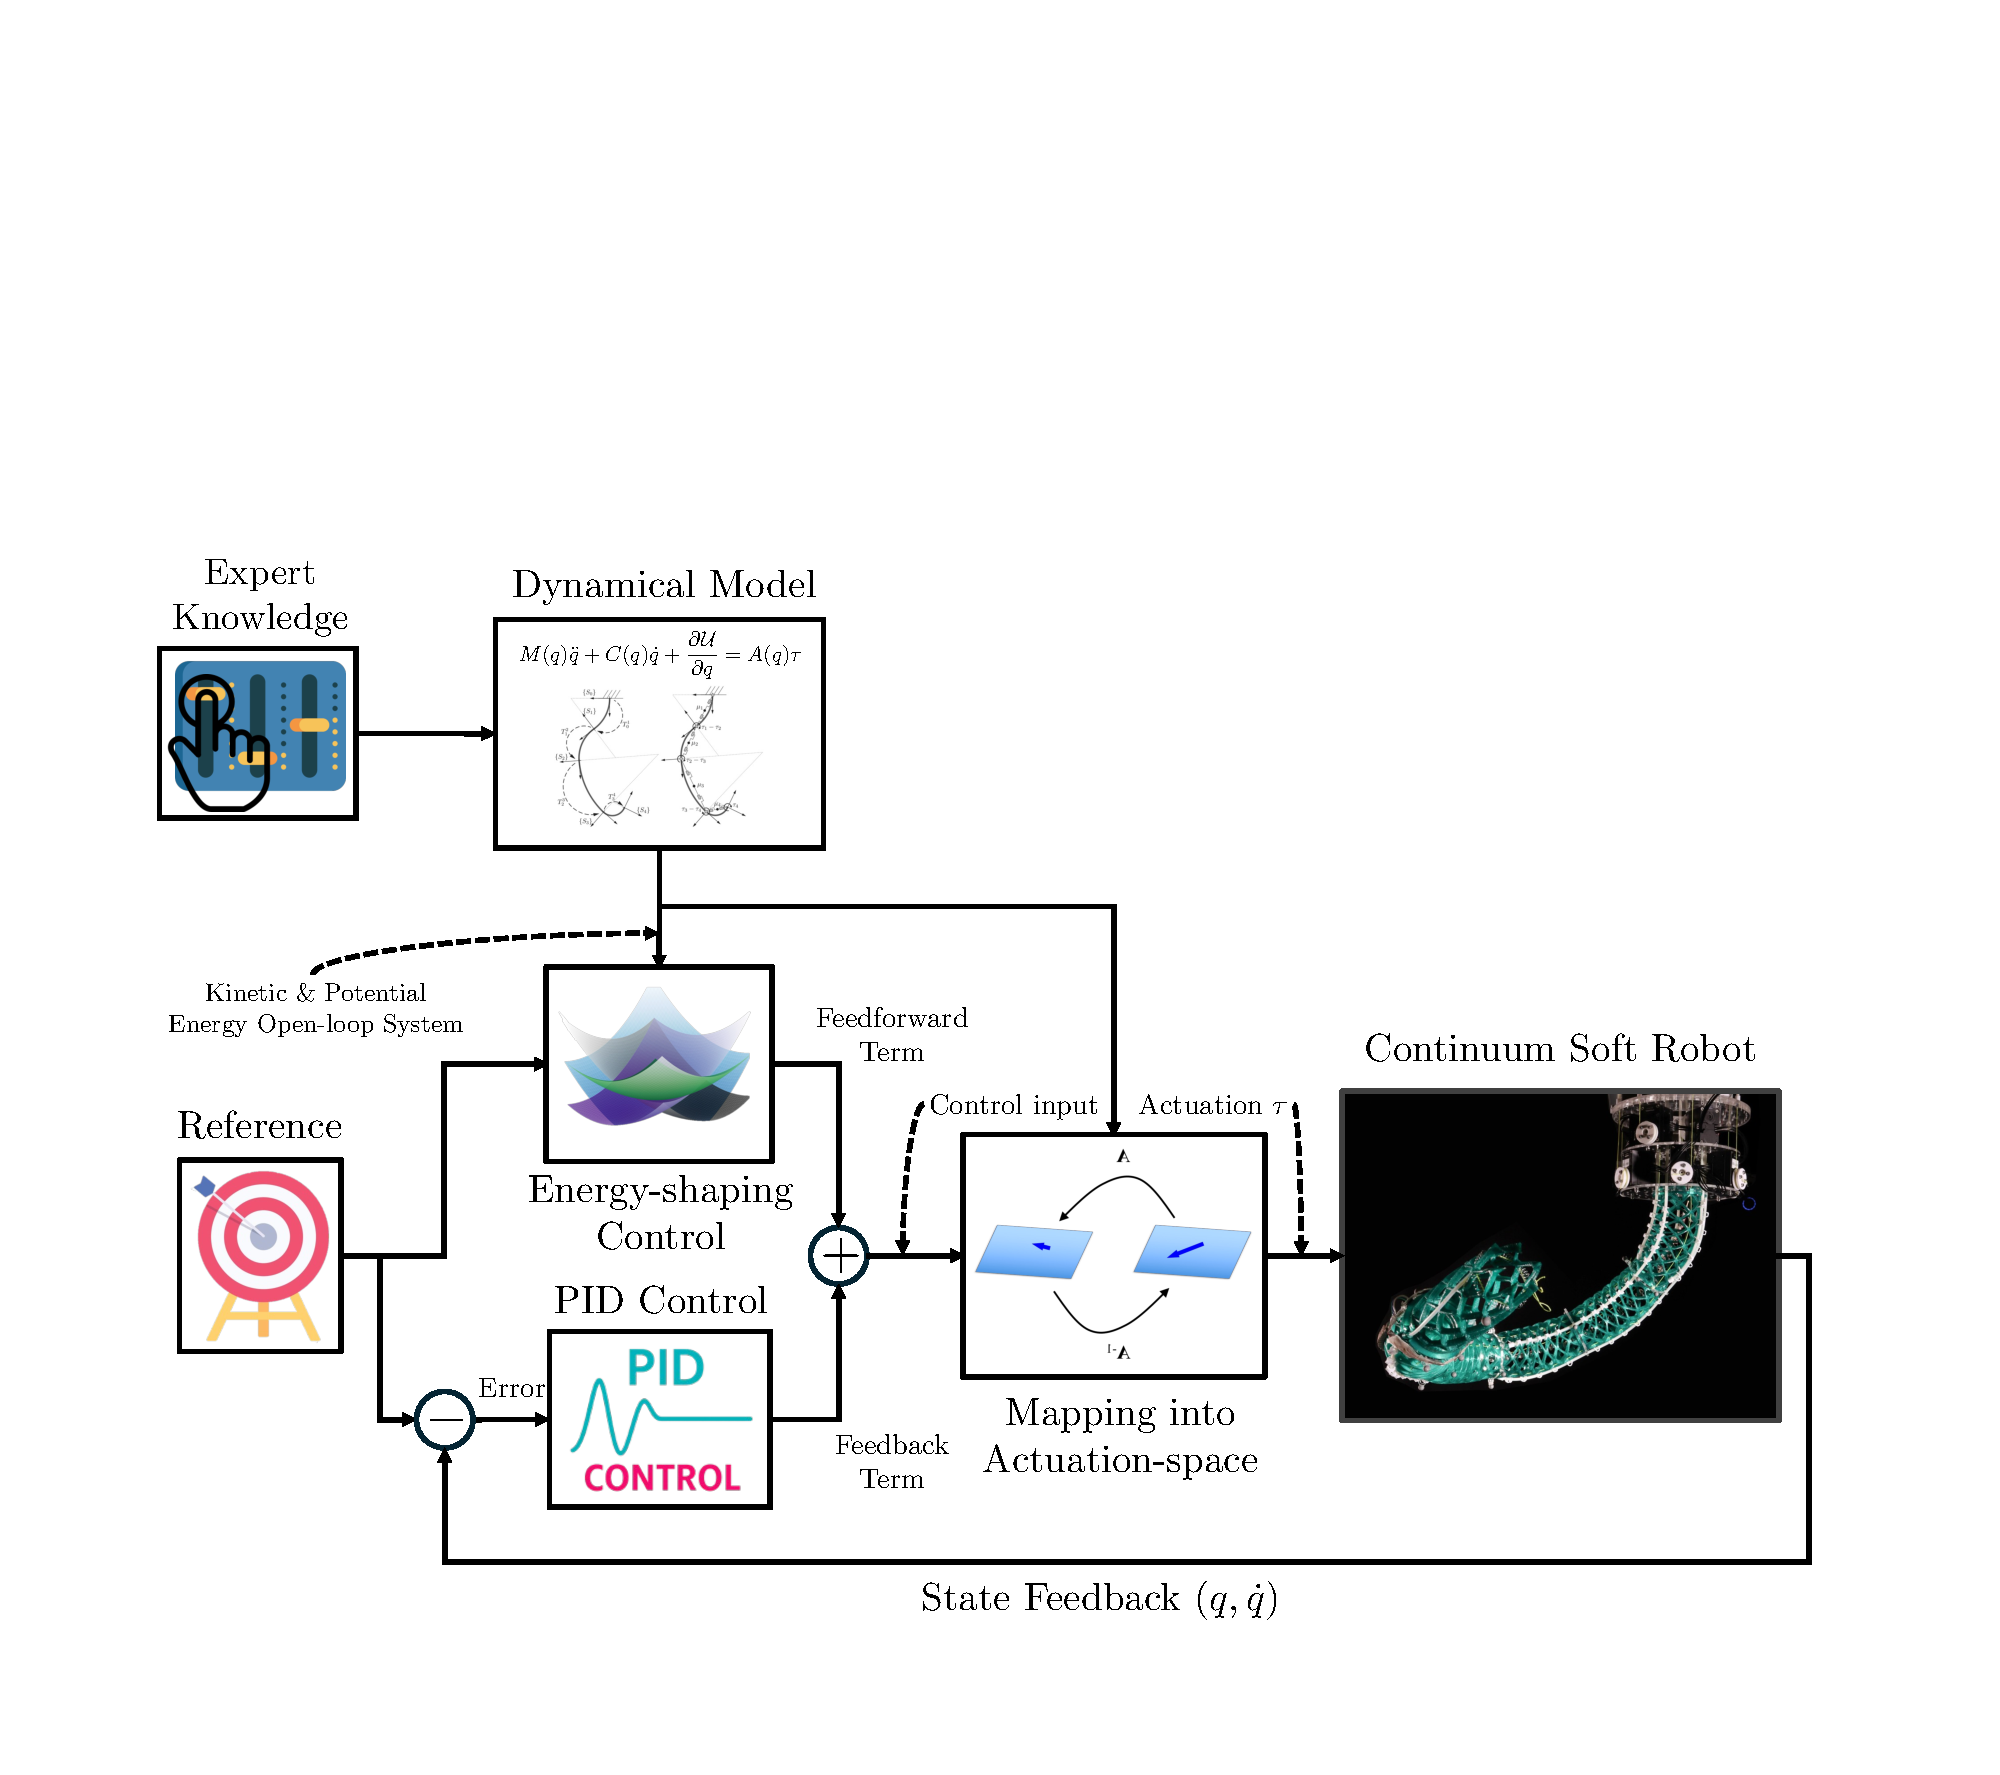
\includegraphics[width=0.49\linewidth]{introduction/figures/model_based_control_with_physical_models_v1_cropped.pdf}\label{fig:introduction:model_based_control_with_physical_models}}\\
%     \subfigure[Learning the Controller]{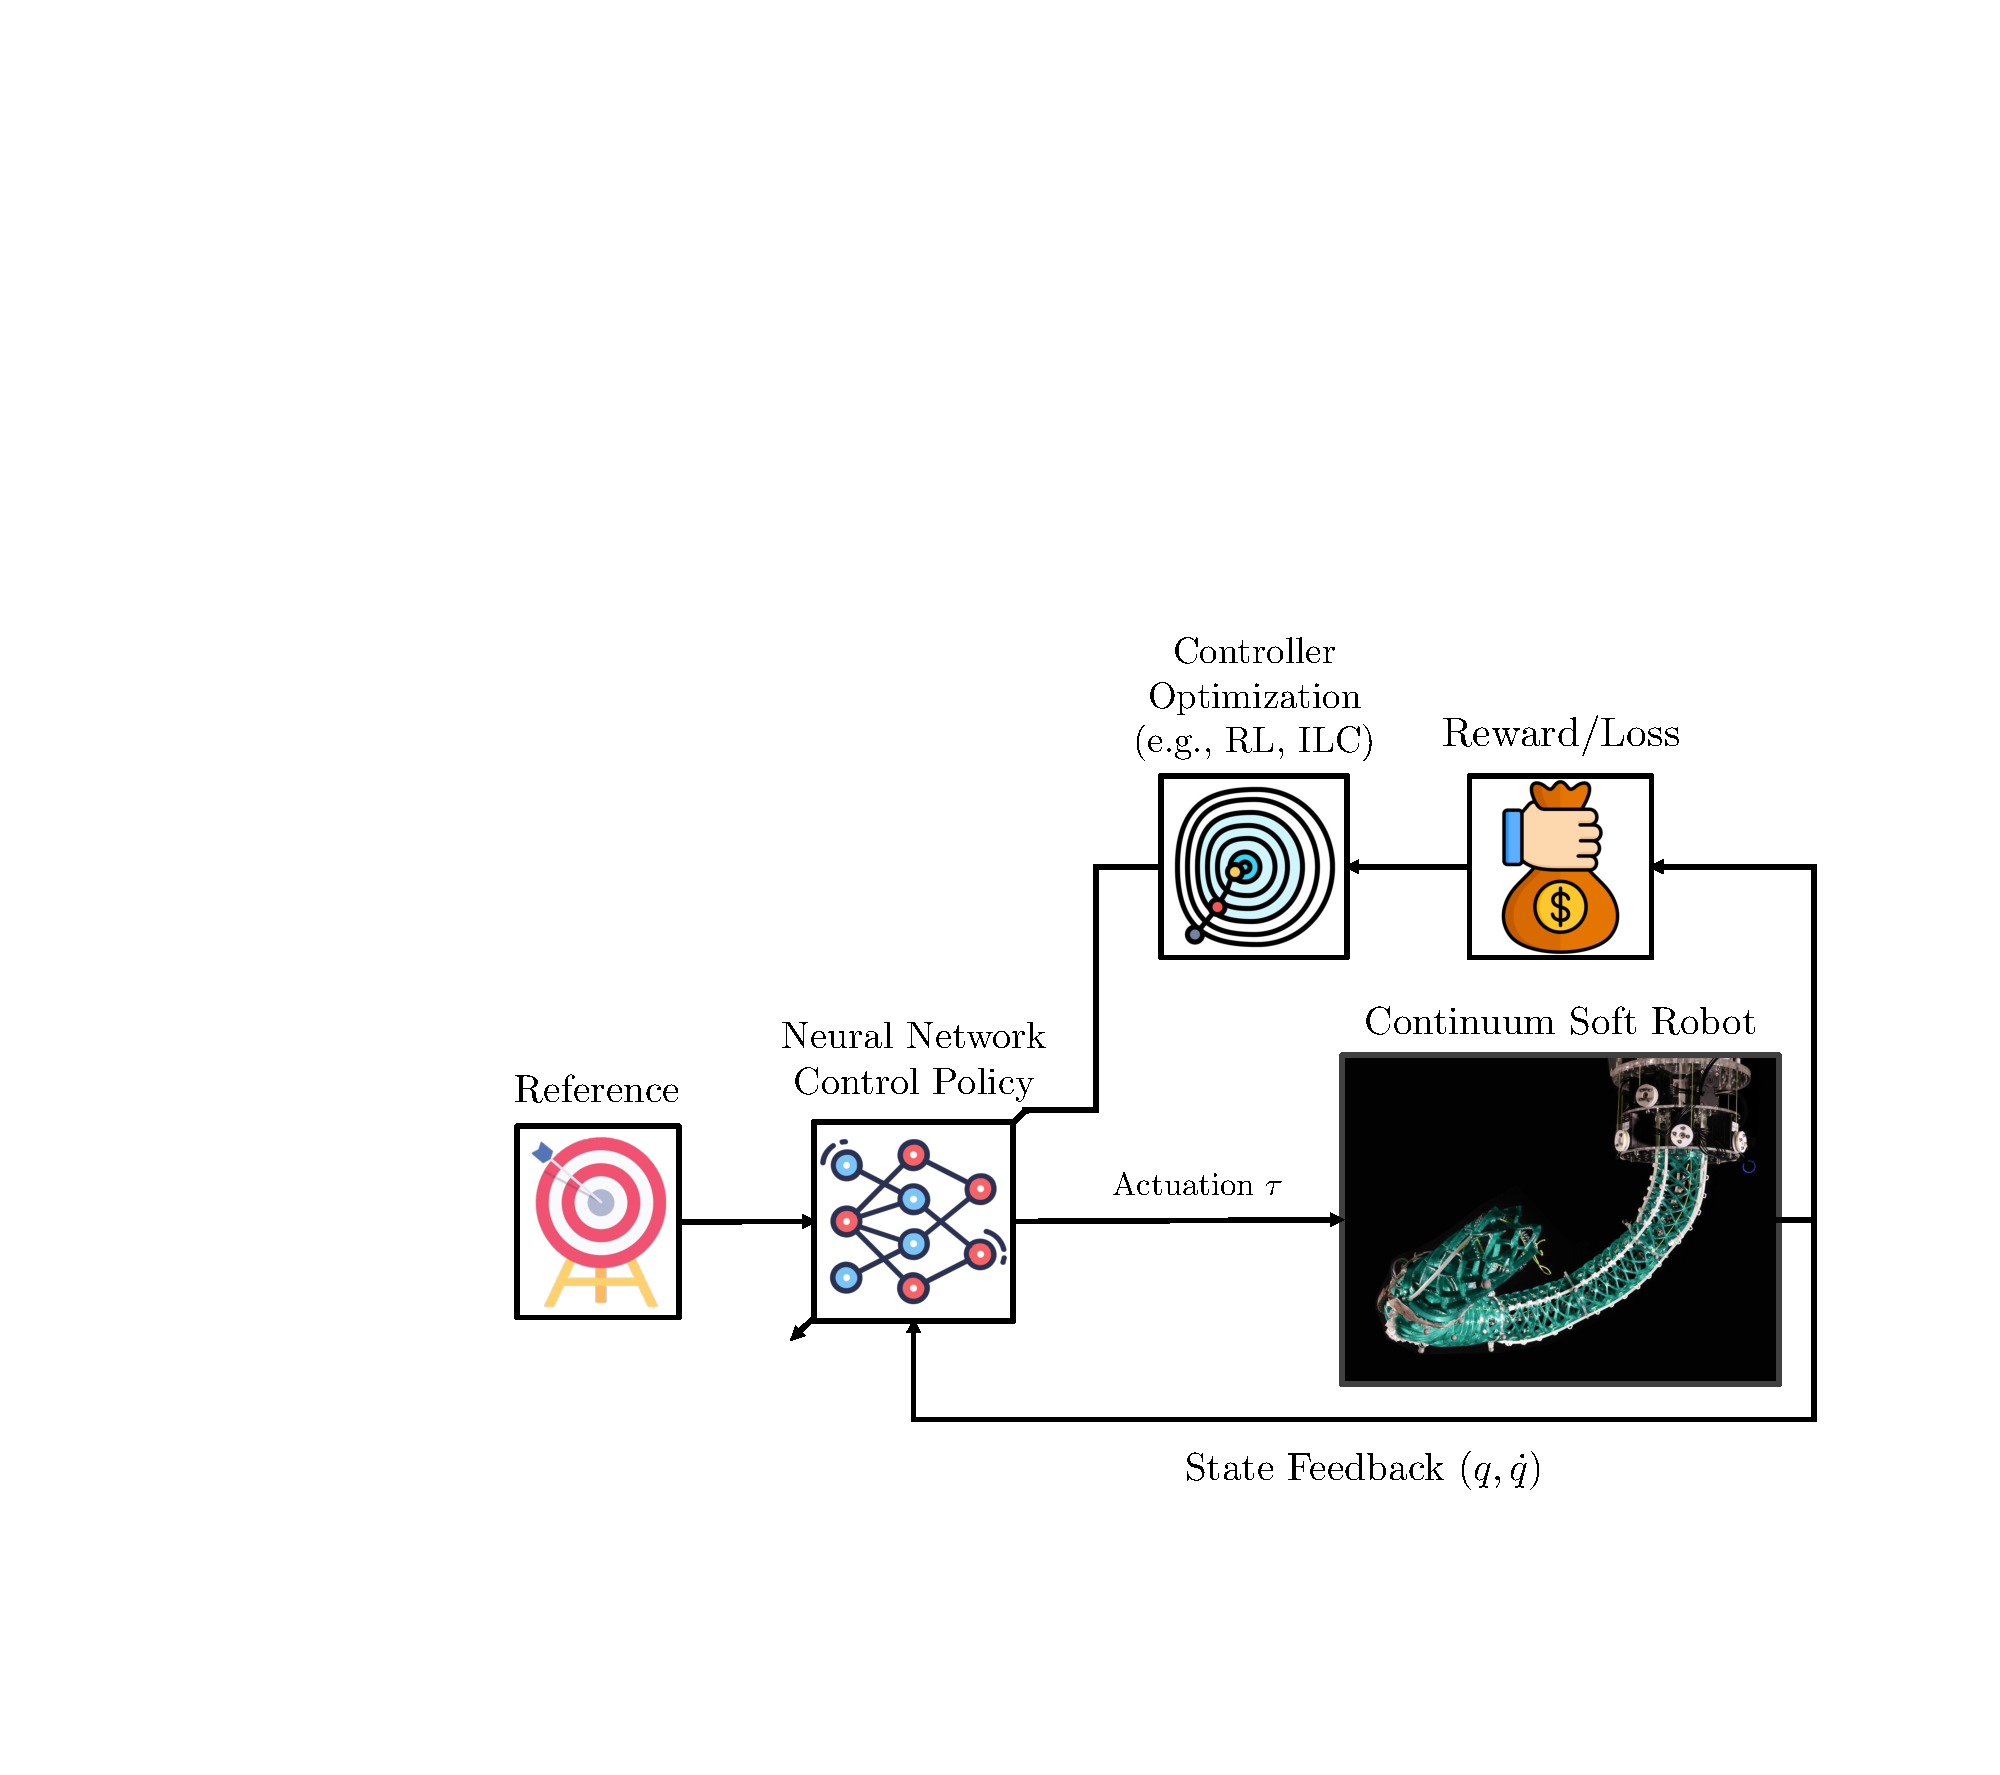
\includegraphics[width=0.44\linewidth]{introduction/figures/controller_learning_v1_cropped.pdf}\label{fig:introduction:direct_controller_learning}}
%     \hfill
%     \subfigure[Closed-form Control with Learned Models]{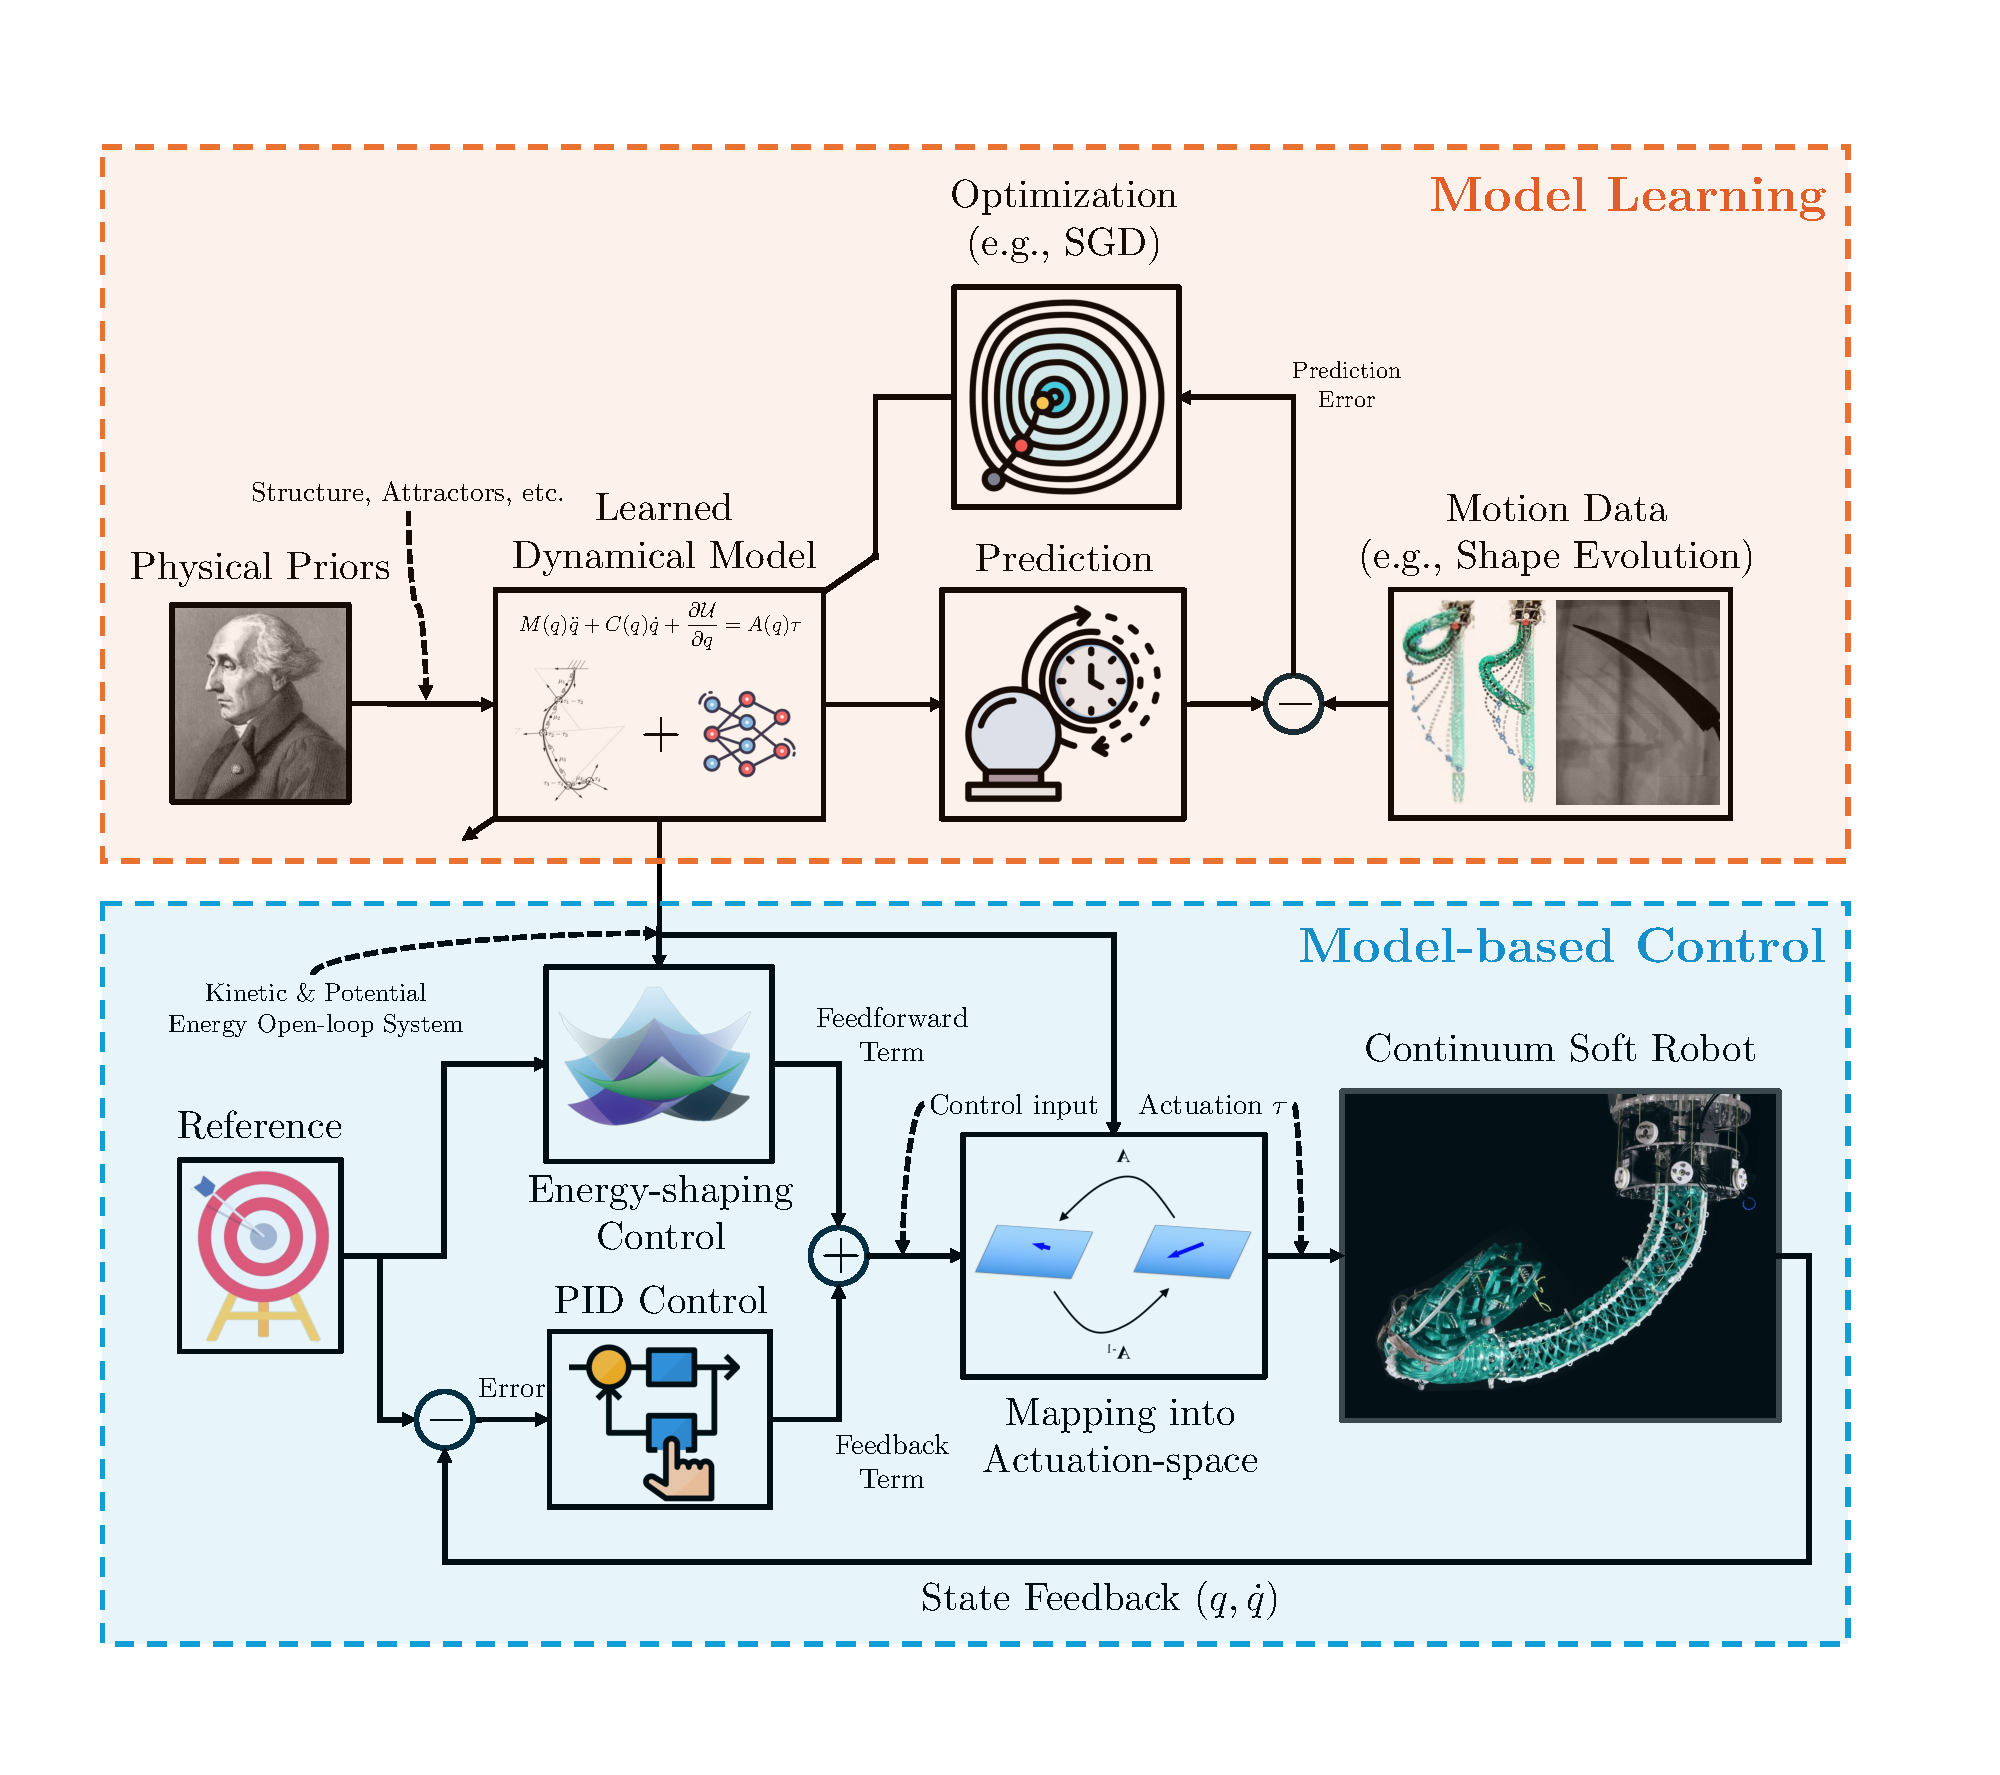
\includegraphics[width=0.50\linewidth]{introduction/figures/model_based_control_with_learned_models_v2_cropped.pdf}\label{fig:introduction:model_based_control_with_learned_models}}
%     \caption{Overview of existing soft robot control approaches (Panels (a)-(c)) and the control strategy proposed in this thesis (Panel (d)).
%     \textbf{Panel (a):} Derivation of physical models from first principles and subsequent usage within closed-form model-based control schemes, such as PID+energy-shaping~\cite{della2023model}.
%     \textbf{Panel (c):} Directly learning the controller via \gls{RL}~\citep{morimoto2021model, jitosho2023reinforcement, alessi2024pushing} or \gls{ILC}~\citep{hofer2019iterative, pierallini2023provably} by interacting with the soft robotic system and optimizing the control policy based on reward/loss/error signals.
%     }
%     \label{fig:introduction:soft_robot_control_approaches}
% \end{figure}

% In this thesis, we aim to avoid all these deficiencies by combining learned models with closed-form control (see Fig.~\ref{fig:introduction:model_based_control_with_learned_models}).
% By integrating learned models into established feedback+feedforward control strategies, we combine the best of both worlds: learning models require less expert knowledge and allow us to capture mode complex dynamical effects while the closed-form feedback+feedforward controller is computationally extremely efficient.
% However, in order to apply feedback+feedforward control strategies, such as PD+energy-shaping~\citep{della2023model, caasenbrood2023control}, we need to be able to inspect the kinetic and potential energies of the learned model, which is generally not possible for existing popular \gls{ML} architectures such as \glspl{RNN}, \glspl{MLP}, or \glspl{NODE}.
% Therefore, we notice that the learned models need to exhibit a physical structure in order for us to be able to apply common model-based control schemes, such as PD+ or PD+feedforward, and to guarantee the stability of the closed-loop system using Lyapunov arguments.
In this thesis, we seek to circumvent the aforementioned shortcomings by integrating learned models with closed-form control, as visualized in Fig.~\ref{fig:introduction:topics_venn}. By embedding learned models within established closed-form model-based control strategies, such as nonlinear feedback~\citep{della2020model} or error-based feedback+energy shaping~\citep{della2023model, caasenbrood2023control}, as visualized in Fig.~\ref{fig:introduction:model_based_control_with_learned_models}, we benefit from both paradigms: learned models demand less specialized expertise while capturing more complex dynamical behaviors, and the closed-form model-based controller remains computationally very efficient. However, to apply such approaches, it is necessary to inspect the kinetic and potential energies of the learned model—something that existing popular \gls{ML} architectures like \glspl{RNN}, \glspl{MLP}, or \glspl{NODE} generally do not allow. Consequently, it becomes clear that the learned models must exhibit a physical structure in order to employ common closed-form model-based control schemes and to secure closed-loop stability via Lyapunov arguments.

% In recent years, there has been an exciting development in this area with the nascent literature on \glspl{LNN}~\citep{lutter2019deep, cranmer2020lagrangian, liu2024physics} and \glspl{HNN}~\citep{greydanus2019hamiltonian, liu2024physics} which both explicitly learn the kinetic and potential energy of the system. However, they also exhibit significant drawbacks: the derivation of the \gls{EOM} requires the online computation of higher-order derivatives, which is computationally expensive (particularly during training but also during inference) and increases (GPU) memory requirements~\citep{lutter2019deep}. Furthermore, in a naive implementation, they do not exhibit any formal stability guarantees, and the computation of higher-order derivatives can introduce numerical stiffness or instability if not carefully managed (e.g., needing high-precision auto differentiation~\citep{rumelhart1986learning} or careful hyperparameter tuning). Finally, we identify a need for learning models that incorporate inductive biases on the specific dynamics exhibited by soft robots.
Recent advances in this direction include the emerging literature on \glspl{LNN}~\citep{lutter2019deep, cranmer2020lagrangian, liu2024physics} and \glspl{HNN}~\citep{greydanus2019hamiltonian, liu2024physics}, both of which explicitly learn the system’s kinetic and potential energies. Nevertheless, these approaches still present substantial challenges: deriving the \gls{EOM} necessitates real-time higher-order derivatives, which is computationally demanding—particularly during training, but also at inference—and escalates (GPU) memory usage~\citep{lutter2019deep}. Moreover, without careful implementation, they do not offer formal stability guarantees, and the computation of higher-order derivatives can cause numerical stiffness or instability~\citep{greydanus2019hamiltonian} unless managed through precise auto-differentiation~\citep{rumelhart1986learning} or meticulous hyperparameter tuning. Finally, there is a clear need for learned models with additional inductive bias tailored to the specific dynamics of soft robots.

% In conclusion, we tackle in this thesis the problem setting of achieving closed-form control of soft robots, ensuring both precise and safe behavior. The key research challenge here is to integrate physical structure into learned models in order to allow exploitation via established PID-like+energy-shaping controllers and stability analysis via Lyapunov arguments.
In conclusion, this thesis addresses the central challenge of achieving closed-form control of soft robots while maintaining accurate and safe operation. The key research goal is to advance our understanding of the physical structure of soft robots and incorporate it into learned models, thereby enabling the use of effective closed-form controllers and allowing for stability verification via Lyapunov-based methods. In the following section, we will pose the principal research question directly connecting to this identified challenge.

